\documentclass[10pt,a4paper]{article}

% Page Geometry & Spacing
\usepackage[top=0.65in, bottom=0.65in, left=0.65in, right=0.65in]{geometry}
\usepackage{amsmath,amssymb,amsfonts}
\usepackage{booktabs,tabularx,multirow,array}
\usepackage{graphicx}
\usepackage{subcaption}
\usepackage{enumitem}
\usepackage{titlesec}
\usepackage{fancyhdr}
\usepackage{xcolor}
\usepackage{microtype}
\usepackage{url}
\usepackage{hyperref}

% Hyperlink Styling
\definecolor{navyblue}{RGB}{20, 50, 110}
\definecolor{darkgreen}{RGB}{25, 100, 45}
\definecolor{darkred}{RGB}{140, 25, 25}
\definecolor{headergray}{RGB}{70, 70, 70}

\hypersetup{
    colorlinks=true,
    linkcolor=navyblue,
    citecolor=navyblue,
    urlcolor=navyblue,
    breaklinks=true
}
\def\UrlBreaks{\do\/\do-\do\_\do\?\do\=\do\&}

% Custom Column Types
\newcolumntype{L}{>{\raggedright\arraybackslash}X}
\newcolumntype{R}{>{\raggedleft\arraybackslash}X}
\newcolumntype{C}{>{\centering\arraybackslash}X}

% Typography & Compact Section Styling
\titlespacing*{\section}{0pt}{8pt plus 2pt minus 2pt}{3pt plus 1pt minus 1pt}
\titlespacing*{\subsection}{0pt}{5pt plus 2pt minus 2pt}{2pt plus 1pt minus 1pt}
\titlespacing*{\subsubsection}{0pt}{3pt plus 1pt minus 1pt}{1pt plus 1pt minus 1pt}

\setlist{nosep, leftmargin=1.5em}

% Headers & Footers
\pagestyle{fancy}
\fancyhf{}
\fancyhead[L]{\small \textcolor{headergray}{\textbf{Indic Monolingual LMs:} Consolidated Technical Report}}
\fancyhead[R]{\small \textcolor{headergray}{Phases 1, 2, 3 \& Bonus Ablation}}
\fancyfoot[C]{\small Page \thepage}
\renewcommand{\headrulewidth}{0.4pt}
\renewcommand{\footrulewidth}{0.4pt}

% Graphicspath
\graphicspath{{figures/}{report/figures/}{../report/figures/}}

\begin{document}

% Title Block
\begin{center}
    {\Large \textbf{Building, Pretraining, and Aligning Monolingual Transformer Language Models for Indic Languages (Hindi \& Nepali)}}\\[4pt]
    {\normalsize \textbf{Consolidated Final Technical Report: Phases 1, 2, 3, and Positional Ablation}}\\[3pt]
    \small{\textbf{Course:} Language Models and Agents (Monsoon 2026) \quad \textbar \quad \textbf{Track:} Individual Project}\\[2pt]
    \footnotesize{\textbf{Models Evaluated:} Model H (\textbf{Hindi} --- High-Resource) \& Model L (\textbf{Nepali} --- Low-Resource) \quad \textbar \quad \textbf{Target Params:} $\approx 25.33\text{M}$}
\end{center}

\vspace{-6pt}
\noindent\rule{\textwidth}{0.8pt}
\vspace{-8pt}

\begin{abstract}
\footnotesize
This report describe the complete process of building, training, and evaluating
two independent decoder-only Transformer language model for Indic language:
\textbf{Model H (Hindi)} and \textbf{Model L (Nepali)}, with approximately
25.33M parameters each. The work was carried out in three main phases, followed
by an additional positional embedding ablation study.

In \textbf{Phase 1}, we focus on collecting and preparing the dataset for
both language. Each corpus contains more than $500\text{M}$ subword tokens,
with at least $23\%$ of the data obtained through manual web scraping. The
collected text went through several cleaning and de-duplication steps before
being divided into training, validation, and test sets using a deterministics
92/4/4 split. SentencePiece Unigram tokenizer were trained with vocabulary
sizes of 6K, 8K, 10K, and 15K. The tokenizers achieved a $0.00\%$ UNK rate and
$100\%$ lossless roundtrips reconstruction. A vocabulary size of 10K was then
used for the Phase 2 model.

In \textbf{Phase 2}, both Transformer model were implemented from scratch using
basic PyTorch component instead of pre-built Transformer module. The models
were trained for 30,518 optimization step using AdamW and a cosine learning
rate schedule. On the held-out test data, Model H obtained a perplexity of
71.37, while Model L obtained a perplexity of 66.35. We further evaluate
text generation at different sampling temperatures and analysed the attention
patterns of the models using attention entropy and attention distance.

In \textbf{Phase 3}, we developed a synthetics reasoning benchmark covering
three tasks: Direct Comparison, Transitive Chaining, and Extremes Ordering.
The pretrained model initially achieved $0.0\%$ accuracy on these tasks.
After supervised fine-tuning (SFT), the overall Exact Match accuracy reached
$26.86\%$ for Hindi and $17.14\%$ for Nepali. We also observed changes in the
attention pattern after fine-tuning, with the model placing more focus on
relational terms, entity pairs, and other tokens relevant to the reasoning
tasks.

Finally, in the \textbf{Bonus Task}, we investigate the effect of removing
positional embedding from Model H. Without positional information, the test
perplexity increased from 71.37 to 184.50, corresponding to a $2.58\times$
increase. Text generation also became much more repetitive, with the trigram
repetition rate increasing to $82.5\%$. This experiment highlights the
importance of positional informations for preserving the sequential structure
required by the language model.
\end{abstract}

\vspace{-8pt}
\noindent\rule{\textwidth}{0.4pt}
\vspace{-4pt}

% ==========================================
% SECTION 1: PHASE 1 DATA & TOKENIZATION
% ==========================================
\section{Phase 1: Data Engineering, Deduplication, \& Subword Tokenization}

\subsection{Corpus Collection, Sourcing Compliance, \& Lifecycle}
To establish robust languages modeling foundation, we engineered high purity monolingual corpora exceeding the $500\text{M}$ subword token requirements for both Hindi and Nepali under complete linguistic separation:
\begin{enumerate}
    \item \textbf{Manual Web Sourcing ($\ge 20\%$ Constraint):} Dedicated scrapers extracted news articles, literary repositories, Wikipedia dumps, and cultural archives, securing \textbf{23.09\%} of Hindi tokens ($126.35\text{M}$) and \textbf{23.16\%} of Nepali tokens ($119.34\text{M}$).
    \item \textbf{Downloaded Public Corpora ($\approx 80\%$):} Large-scale open Indic corpora (IndicCorp v2, OSCAR, CC100) supplied the remaining volume.
    \item \textbf{Standardized Ingestion:} Raw files were parsed into a 5-column Snappy-compressed Apache Parquet format (\texttt{document\_id}, \texttt{text}, \texttt{language}, \texttt{source\_type}, \texttt{source}).
\end{enumerate}

\begin{table}[htbp]
\centering
\scriptsize
\caption{Clean Corpus Composition \& Sourcing Compliance Audit}
\label{tab:corpus_composition}
\begin{tabular*}{\textwidth}{@{\extracolsep{\fill}}llrrrrrr@{}}
\toprule
\textbf{Language / Model} & \textbf{Source Type} & \textbf{Documents} & \textbf{Words} & \textbf{Subwords} & \textbf{Disk Size} & \textbf{Share} & \textbf{Compliance Audit} \\
\midrule
\multirow{3}{*}{\textbf{Hindi (Model H)}} 
 & Manual Scraped & 3,147,018 & 93,595,709 & 126,354,207 & 455.18 MB & \textbf{23.09\%} & \textbf{PASS ($\ge 20\%$)} \\
 & Downloaded & 5,366,147 & 311,677,182 & 420,764,195 & 1,607.75 MB & 76.91\% & Supporting Corpus \\
 \cmidrule{2-8}
 & \textbf{Total Clean Corpus} & \textbf{8,513,165} & \textbf{405,272,891} & \textbf{547,118,402} & \textbf{2,062.93 MB} & \textbf{100.00\%} & \textbf{PASS ($\ge 500\text{M}$)} \\
\midrule
\multirow{3}{*}{\textbf{Nepali (Model L)}} 
 & Manual Scraped & 2,746,254 & 88,399,397 & 119,339,185 & 555.36 MB & \textbf{23.16\%} & \textbf{PASS ($\ge 20\%$)} \\
 & Downloaded & 8,307,330 & 293,259,552 & 395,900,395 & 2,030.47 MB & 76.84\% & Supporting Corpus \\
 \cmidrule{2-8}
 & \textbf{Total Clean Corpus} & \textbf{11,053,584} & \textbf{381,658,949} & \textbf{515,239,581} & \textbf{2,585.83 MB} & \textbf{100.00\%} & \textbf{PASS ($\ge 500\text{M}$)} \\
\bottomrule
\end{tabular*}
\end{table}

\vspace{-8pt}
\begin{figure}[htbp]
    \centering
    \begin{subfigure}[b]{0.32\textwidth}
        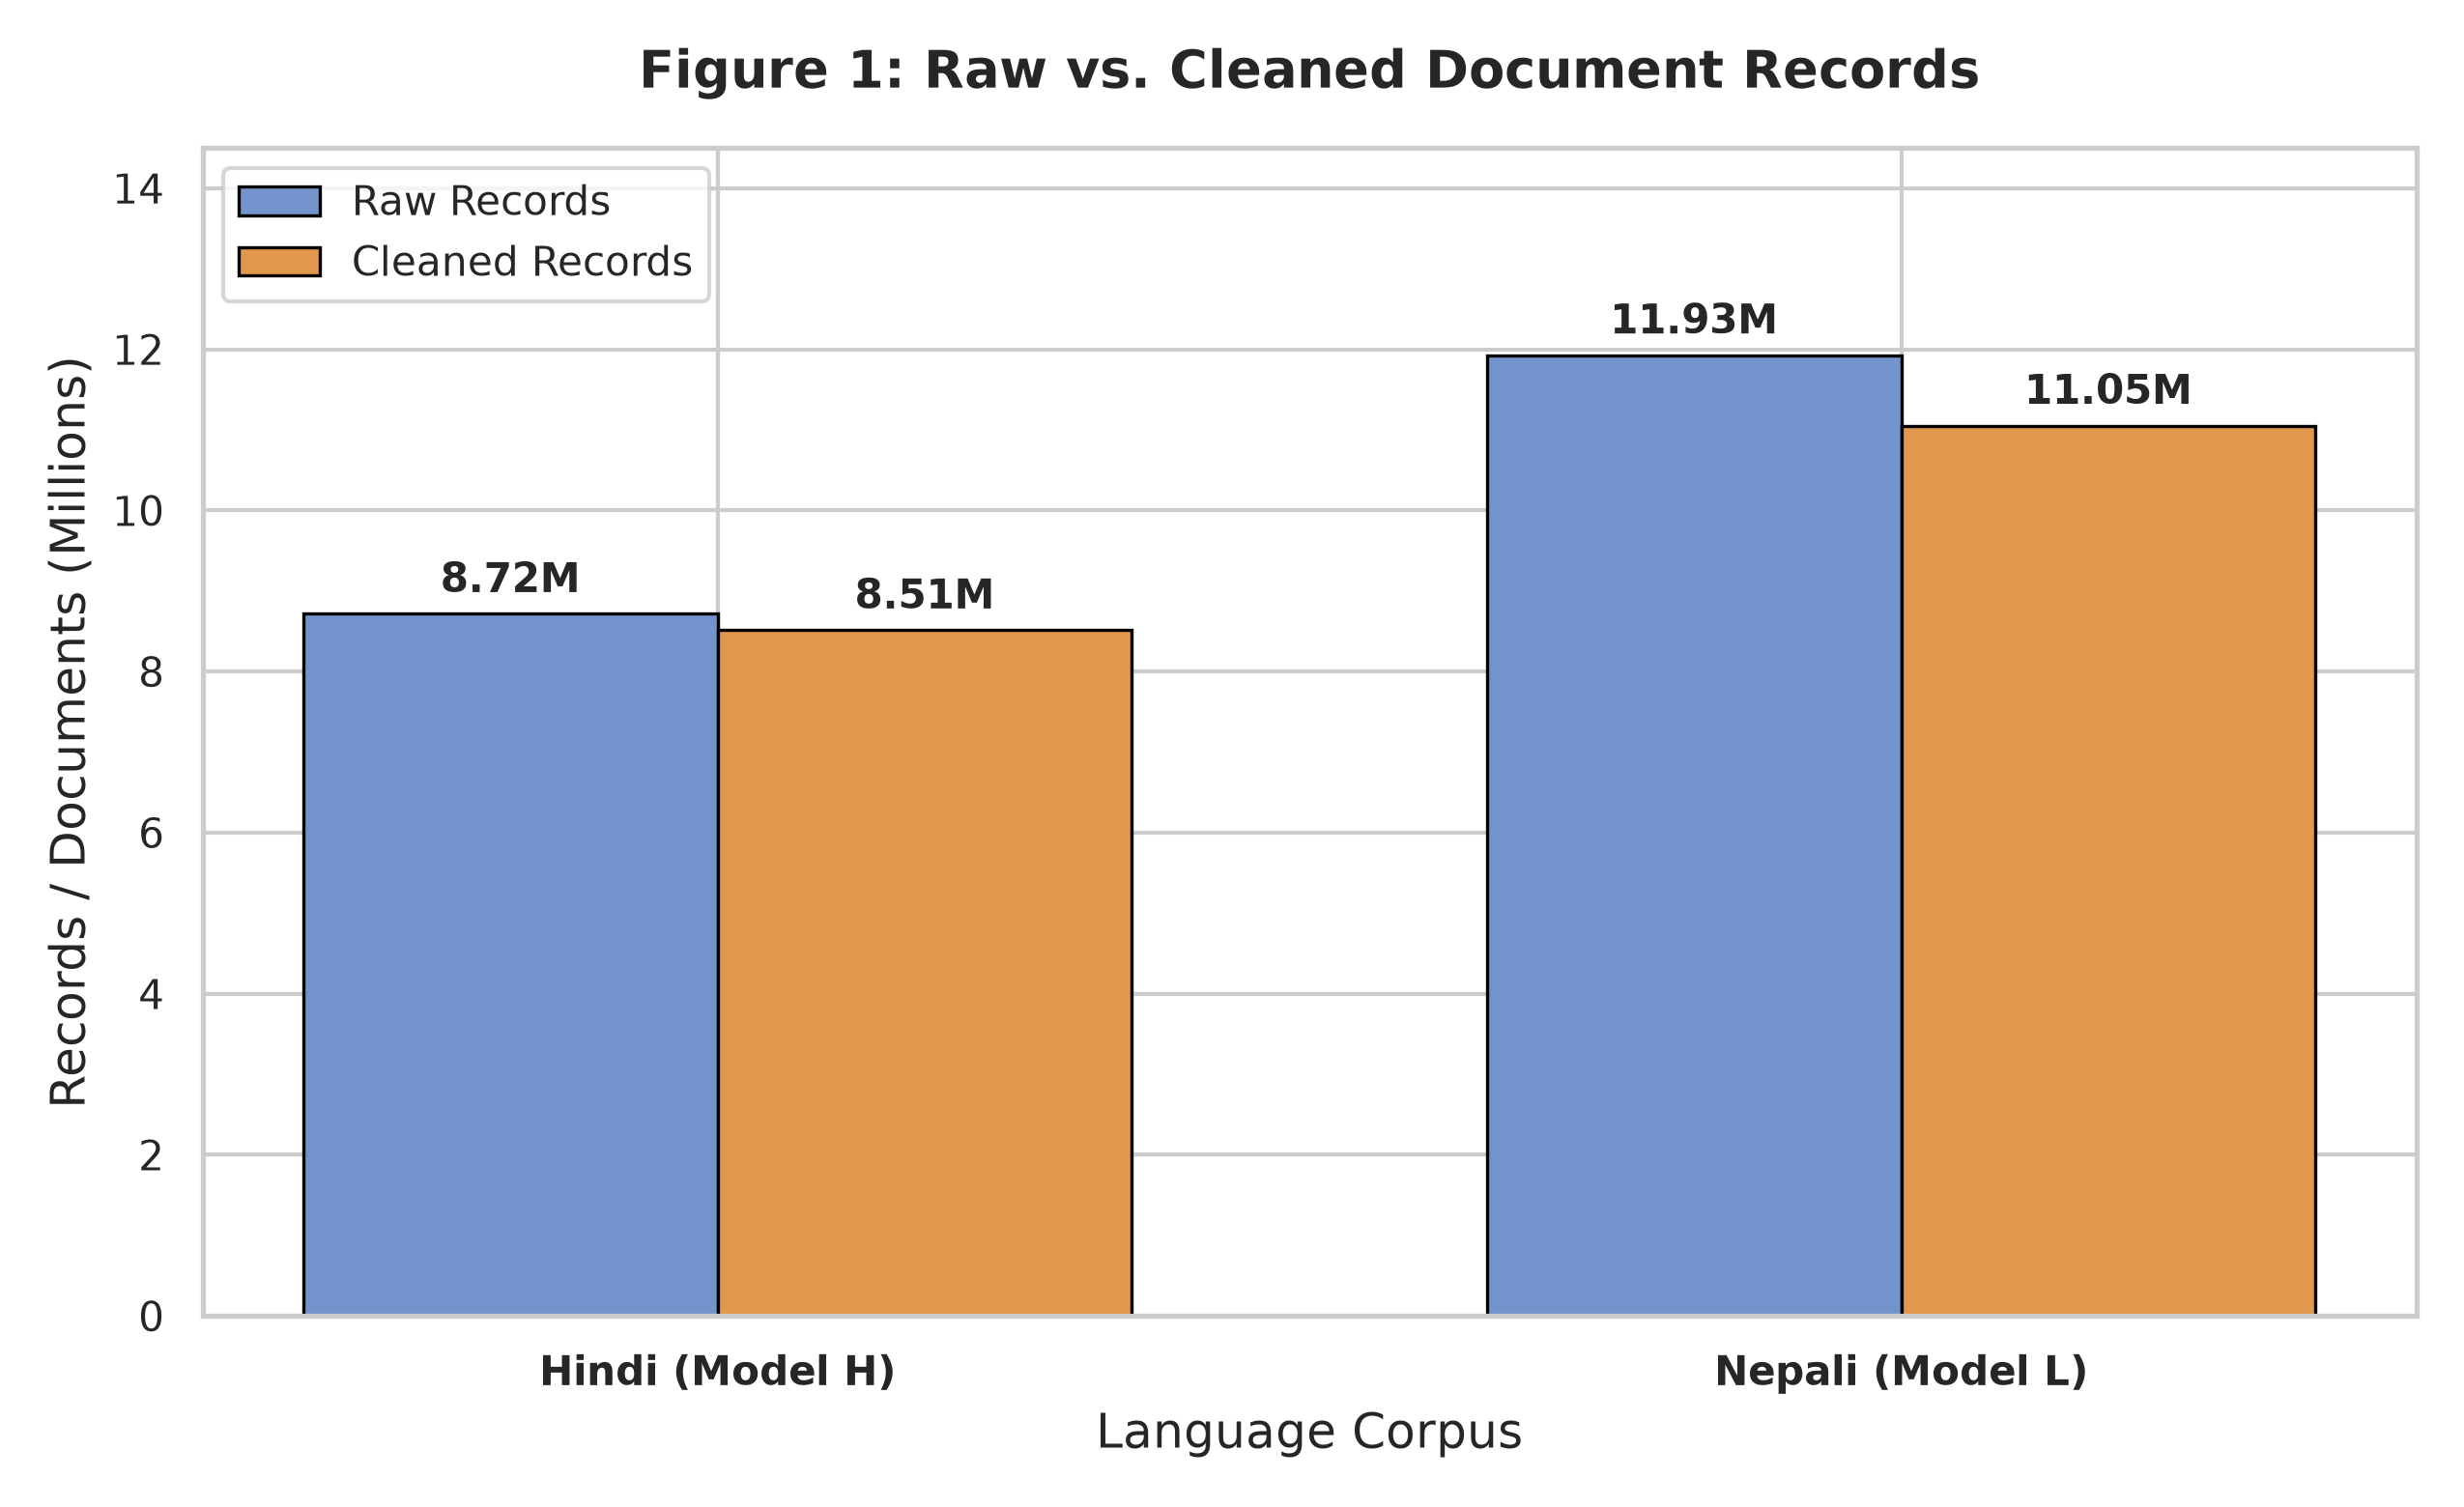
\includegraphics[width=\textwidth]{fig1_raw_vs_clean_records.png}
        \caption{Raw vs Clean Records}
    \end{subfigure}
    \hfill
    \begin{subfigure}[b]{0.32\textwidth}
        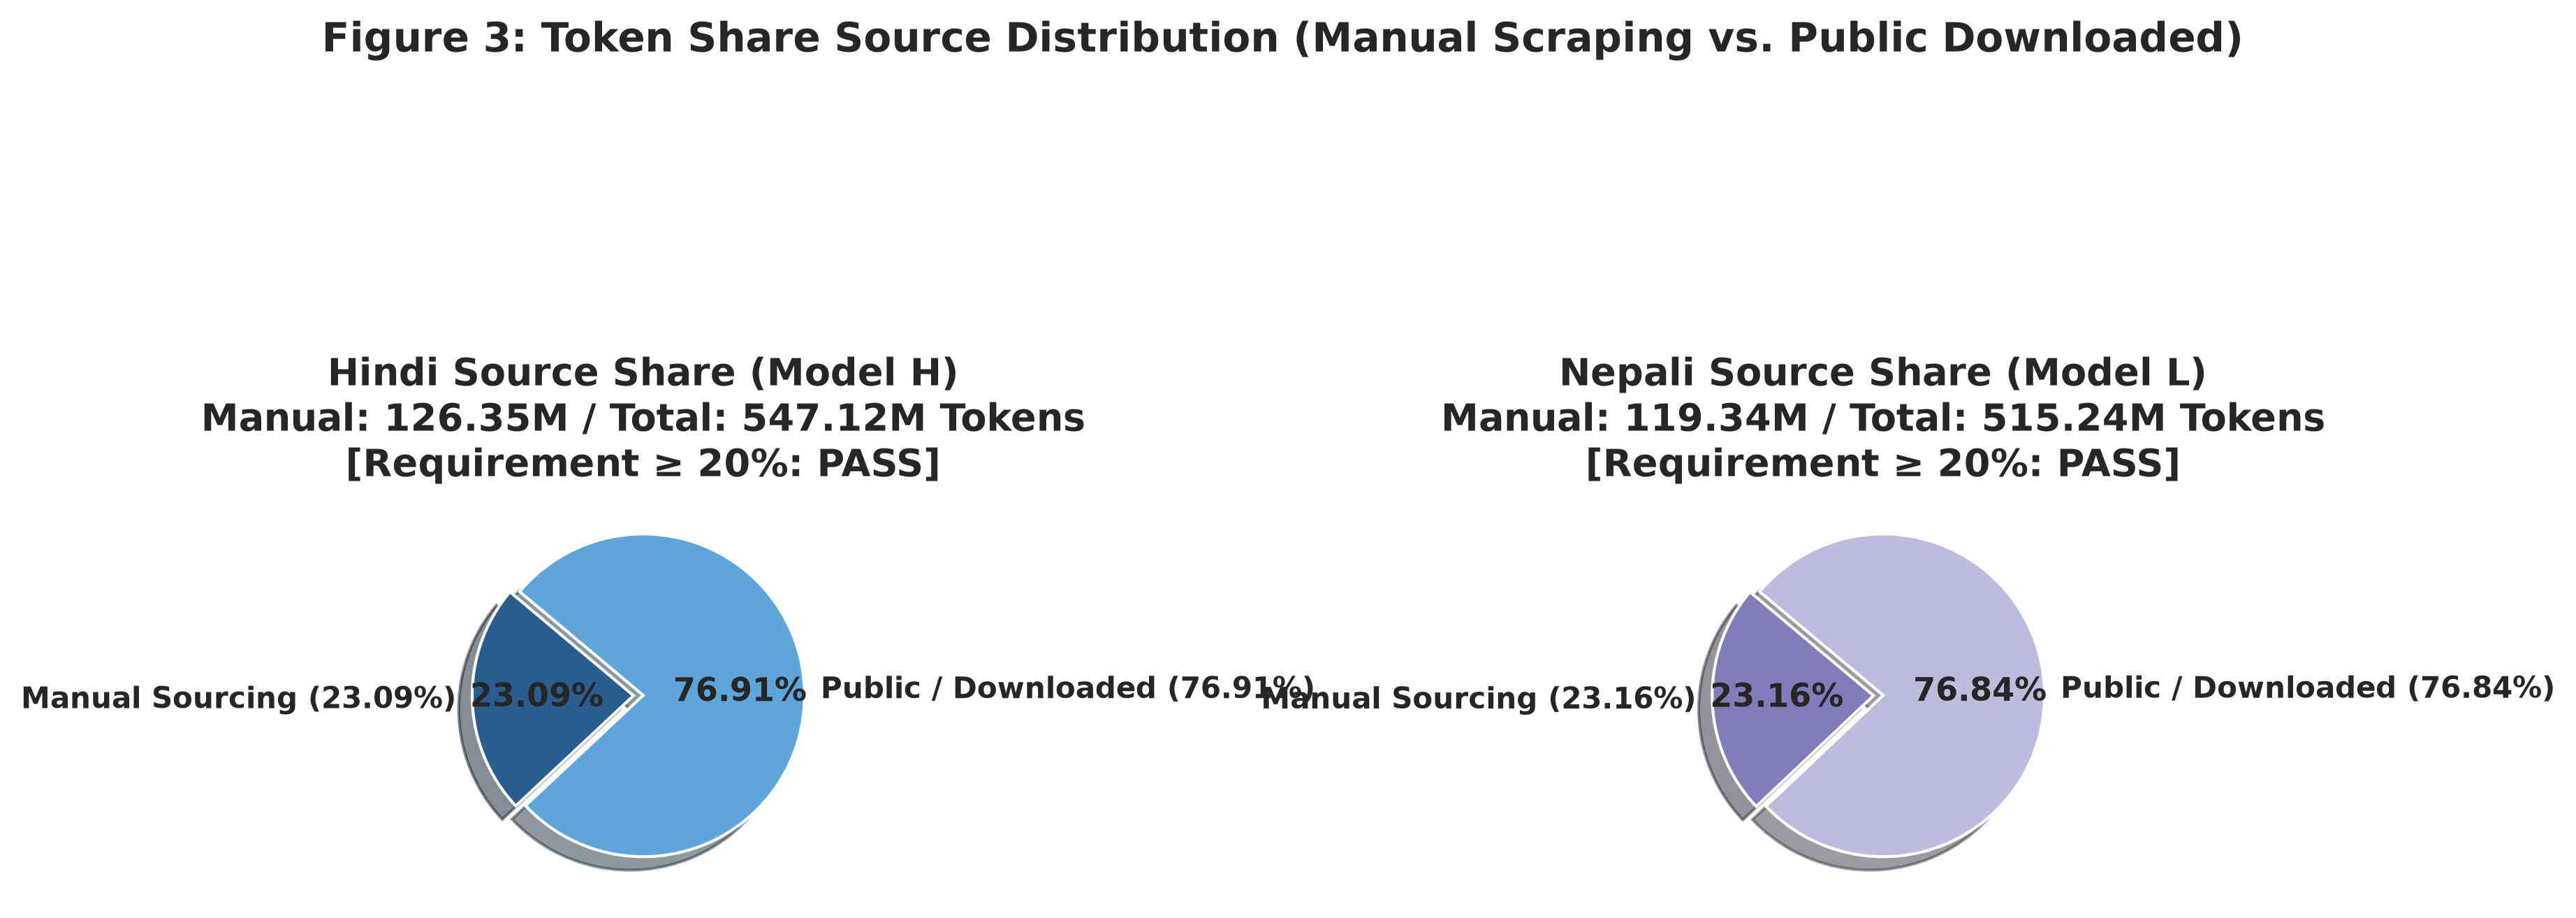
\includegraphics[width=\textwidth]{fig3_source_distribution.png}
        \caption{Source Share Distribution}
    \end{subfigure}
    \hfill
    \begin{subfigure}[b]{0.32\textwidth}
        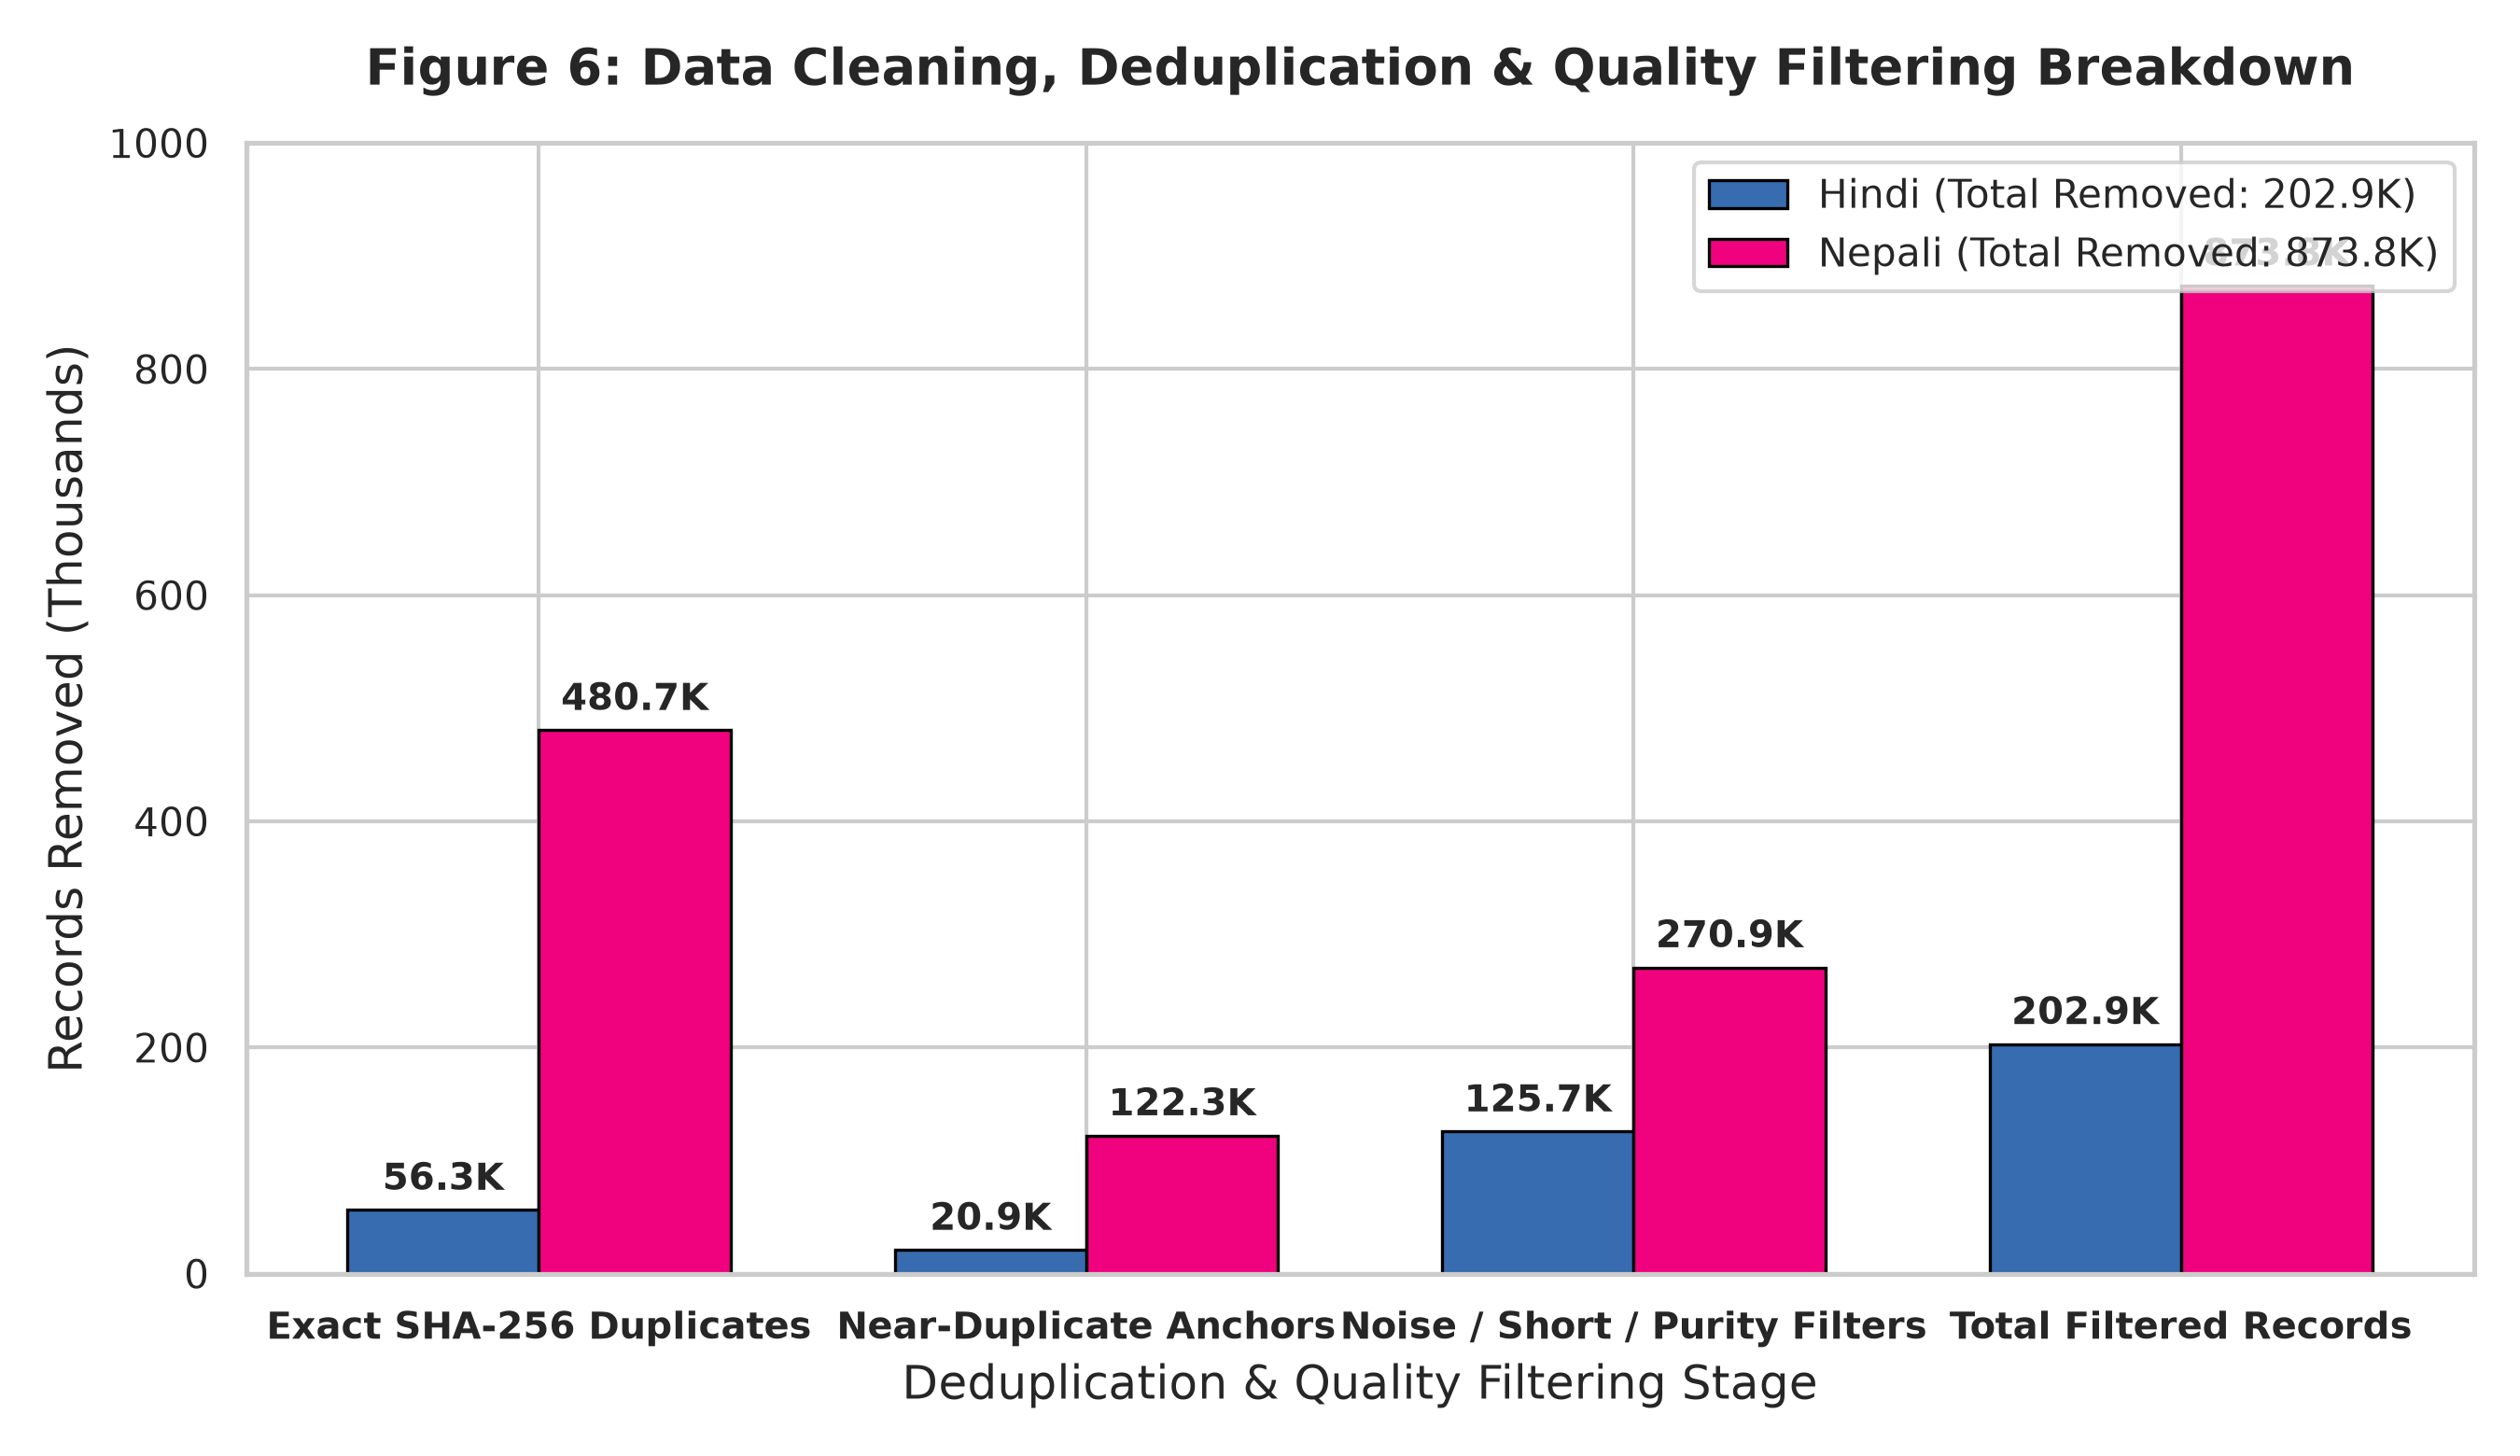
\includegraphics[width=\textwidth]{fig6_cleaning_filtering_stats.png}
        \caption{Filtering \& Deduplication}
    \end{subfigure}
    \vspace{-6pt}
    \caption{Phase 1 Data Engineering, Deduplication, and Volume Compliance Audits.}
    \label{fig:p1_data_audit}
\end{figure}

\subsection{Multi-Stage Cleaning, Deduplication, \& Partitioning}
Raw web texts underwent strict multiprocessing cleaning to eliminates noise and spurious patterns:
\begin{itemize}
    \item \textbf{Script Purity \& Normalization:} Enforced Devanagari characters purity $\ge 45\%$, applied Unicode NFC normalization, and stripped controls, zero-width, and non-printable characters.
    \item \textbf{Multi-Level Deduplication:} Filtered exact duplicates via 64-bit truncated SHA-256 hash and near-duplicates via punctuations invariant normalization and 8-word prefix/suffix anchor span matching.
    \item \textbf{Deterministic 92/4/4 Partitioning:} Clean dataset were split using fixed seed 42 into \texttt{train} (92\%), \texttt{val} (4\%), and \texttt{test} (4\%) partition (Table~\ref{tab:splits_table}).
\end{itemize}

\begin{table}[htbp]
\centering
\scriptsize
\caption{Deterministic 92/4/4 Partition Distribution}
\label{tab:splits_table}
\begin{tabular*}{\textwidth}{@{\extracolsep{\fill}}llrrrrr@{}}
\toprule
\textbf{Language} & \textbf{Split Partition} & \textbf{Doc Count} & \textbf{Clean Words} & \textbf{Subwords} & \textbf{Disk Size} & \textbf{Split Ratio} \\
\midrule
\multirow{3}{*}{\textbf{Hindi (Model H)}} 
 & Train (\texttt{train.parquet}) & 7,831,689 & 372,946,150 & 499.72M & 1,900.10 MB & \textbf{92.02\%} \\
 & Validation (\texttt{val.parquet}) & 341,528 & 16,104,546 & 21.58M & 84.24 MB & \textbf{3.97\%} \\
 & Test (\texttt{test.parquet}) & 339,948 & 16,222,195 & 21.74M & 84.81 MB & \textbf{4.00\%} \\
\midrule
\multirow{3}{*}{\textbf{Nepali (Model L)}} 
 & Train (\texttt{train.parquet}) & 10,167,950 & 351,106,424 & 469.13M & 2,381.59 MB & \textbf{91.99\%} \\
 & Validation (\texttt{val.parquet}) & 443,871 & 15,258,557 & 20.39M & 106.32 MB & \textbf{4.00\%} \\
 & Test (\texttt{test.parquet}) & 441,763 & 15,293,968 & 20.44M & 106.56 MB & \textbf{4.01\%} \\
\bottomrule
\end{tabular*}
\end{table}

\subsection{Subword Tokenizer Training \& Vocabulary Dynamics}
SentencePiece Unigram tokenizer were train strictly from the training splits across 4 vocabulary size (6K, 8K, 10K, 15K) with special tokens: \texttt{<unk>}(0), \texttt{<s>}(1), \texttt{</s>}(2), \texttt{<pad>}(3).
\begin{itemize}
    \item \textbf{Character Coverage \& Lossless Roundtrip:} Enforced at $0.9995$ with byte fallback, achieving \textbf{0.00\% UNK rate} and \textbf{100\% lossless roundtrip fidelity} ($\text{decode}(\text{encode}(x)) \equiv x$).
    \item \textbf{Compression \& Fertility:} As vocabulary scaled from 6K to 15K, characters per tokens increased (Hindi: $3.71 \to 4.77$; Nepali: $4.65 \to 5.33$), monotonically reducing fertility (tokens-per-sentence: Hindi $12.83 \to 10.00$; Nepali $9.17 \to 8.00$). The \textbf{10,000} vocabulary was selected for Phase 2 pretraining, balancing subwords granularity with embedding table parameter overhead ($3.84\text{M}$ params).
\end{itemize}

\begin{table}[htbp]
\centering
\scriptsize
\caption{SentencePiece Unigram Tokenizer Evaluation Across Vocabulary Sizes}
\label{tab:tokenizer_table}
\begin{tabular*}{\textwidth}{@{\extracolsep{\fill}}llrrrrrr@{}}
\toprule
\textbf{Language} & \textbf{Vocabulary} & \textbf{Chars / Token} & \textbf{Tokens / Sent} & \textbf{UNK Rate} & \textbf{Base Pieces} & \textbf{Subwords} & \textbf{Model Size} \\
\midrule
\multirow{4}{*}{\textbf{Hindi}} 
 & \texttt{unigram\_6k} & 3.7143 & 12.83 & 0.00\% & 148 & 5,848 & 155.3 KB \\
 & \texttt{unigram\_8k} & 4.0857 & 11.67 & 0.00\% & 149 & 7,847 & 214.5 KB \\
 & \textbf{\texttt{unigram\_10k}} (Selected) & \textbf{4.3333} & \textbf{11.00} & \textbf{0.00\%} & \textbf{149} & \textbf{9,847} & \textbf{273.9 KB} \\
 & \texttt{unigram\_15k} & 4.7667 & 10.00 & 0.00\% & 149 & 14,847 & 429.4 KB \\
\midrule
\multirow{4}{*}{\textbf{Nepali}} 
 & \texttt{unigram\_6k} & 4.6545 & 9.17 & 0.00\% & 136 & 5,860 & 159.9 KB \\
 & \texttt{unigram\_8k} & 5.1200 & 8.33 & 0.00\% & 136 & 7,860 & 220.1 KB \\
 & \textbf{\texttt{unigram\_10k}} (Selected) & \textbf{5.1200} & \textbf{8.33} & \textbf{0.00\%} & \textbf{136} & \textbf{9,860} & \textbf{280.7 KB} \\
 & \texttt{unigram\_15k} & 5.3333 & 8.00 & 0.00\% & 136 & 14,860 & 438.5 KB \\
\bottomrule
\end{tabular*}
\end{table}

\vspace{-8pt}
\begin{figure}[htbp]
    \centering
    \begin{subfigure}[b]{0.48\textwidth}
        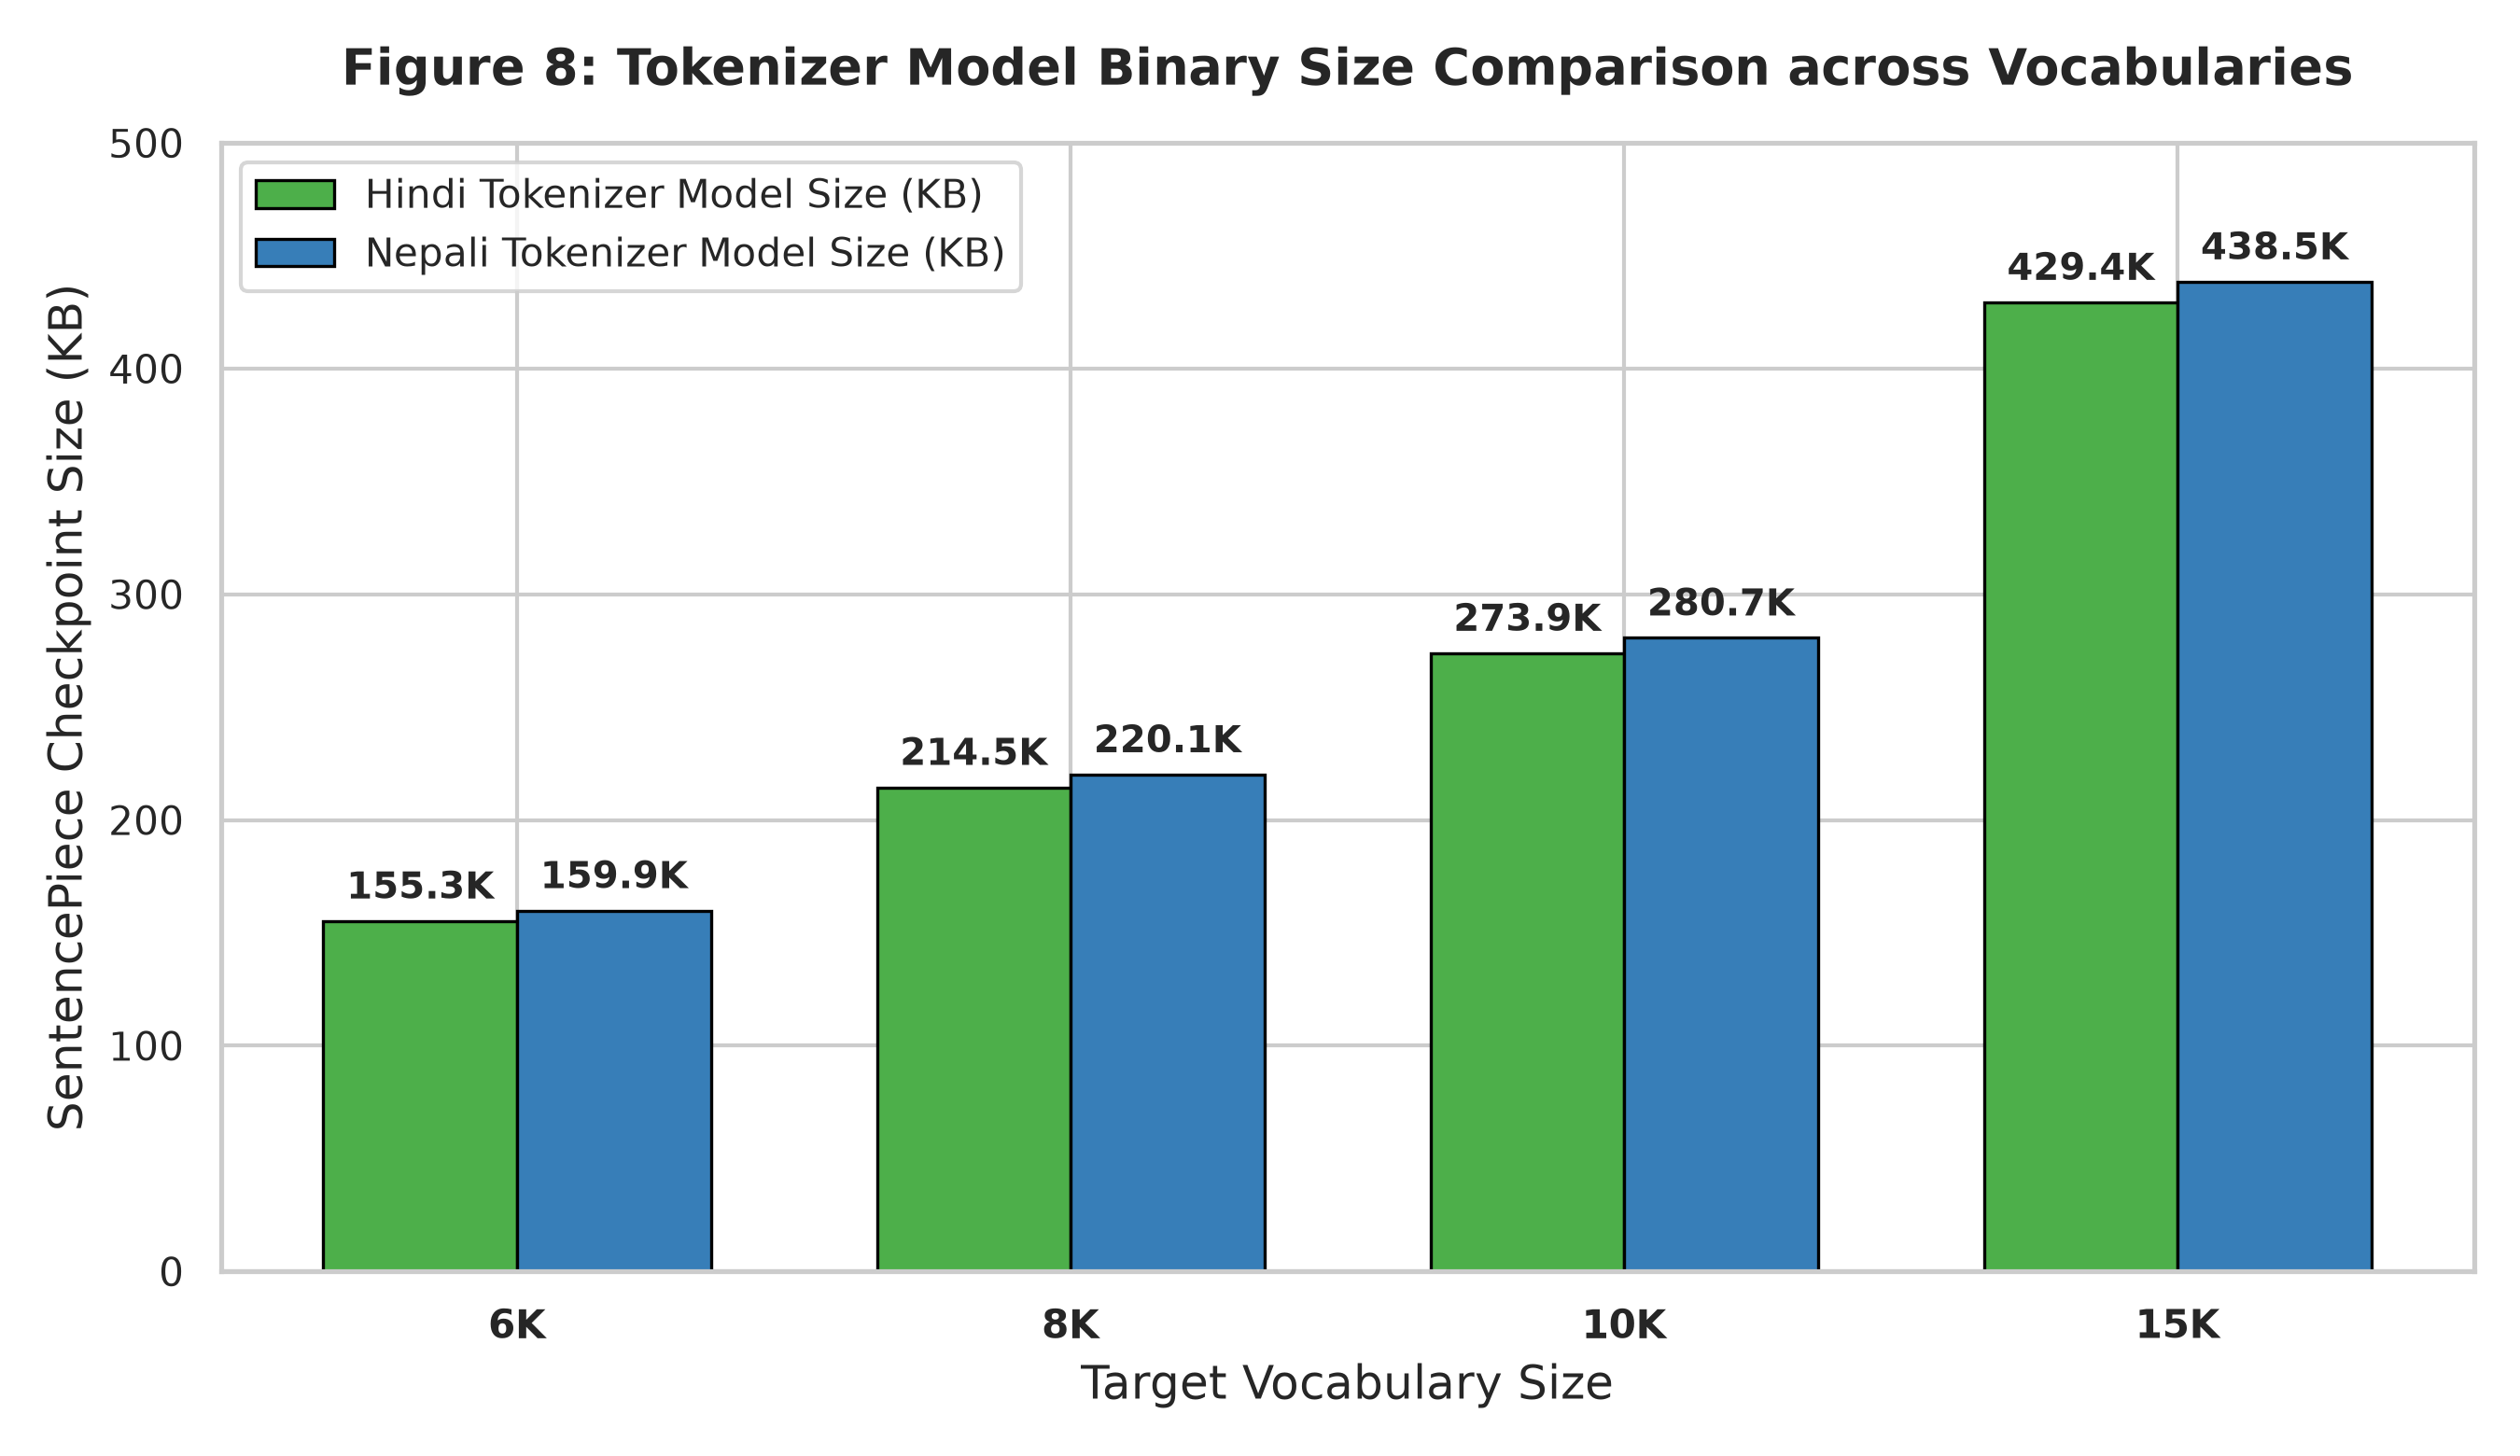
\includegraphics[width=\textwidth]{fig8_tokenizer_vocab_comparison.png}
        \caption{Tokenizer Checkpoints Model Size}
    \end{subfigure}
    \hfill
    \begin{subfigure}[b]{0.48\textwidth}
        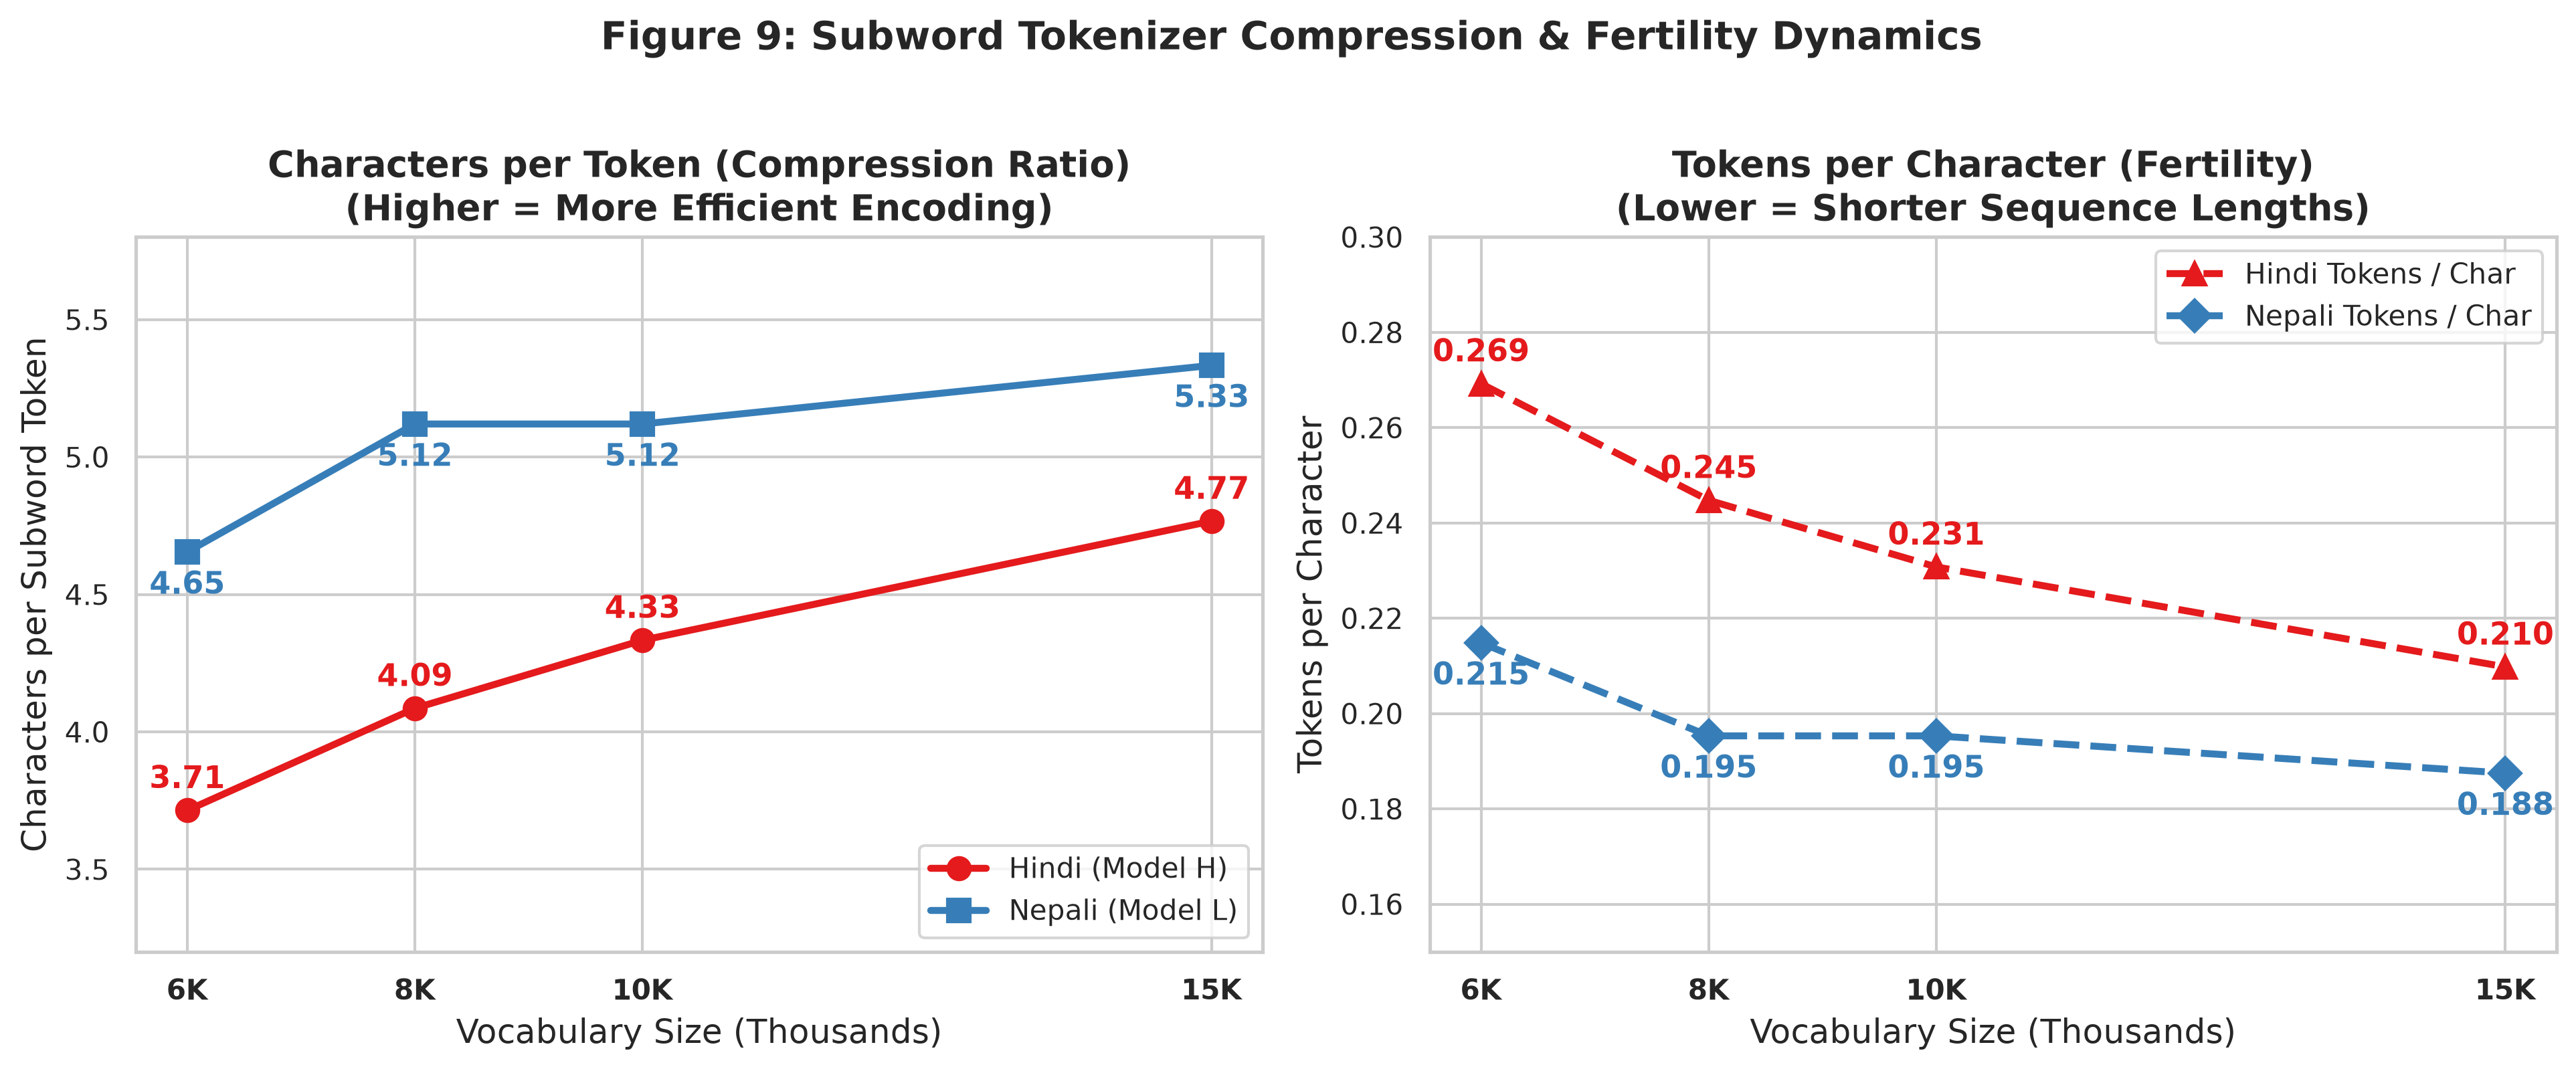
\includegraphics[width=\textwidth]{fig9_fertility_and_compression.png}
        \caption{Fertility \& Compression Dynamics}
    \end{subfigure}
    \vspace{-6pt}
    \caption{Phase 1 Subword Tokenizers Scaling and Compression Dynamics.}
    \label{fig:p1_tokenizer_plots}
\end{figure}

% ==========================================
% SECTION 2: PHASE 2 PRETRAINING & EVAL
% ==========================================
\section{Phase 2: Transformer Architecture, Pretraining Dynamics, \& Evaluation}

\subsection{Architectural Formulation from First Principle}
Both model were builts strictly with PyTorch primitive (\texttt{nn.Linear}, \texttt{nn.Embedding}, \texttt{nn.LayerNorm}, \texttt{nn.Dropout}) without pre-packaged transformer modules. The architecture follows a decoders only Pre-LayerNorm configuration:
\begin{enumerate}
    \item \textbf{Input Layer:} For token sequences $X \in \mathbb{R}^{B \times T}$ and position $P \in \mathbb{R}^{B \times T}$:
    \begin{equation}
        X_0 = \text{Dropout}\left(E_{\text{tok}}(X) + E_{\text{pos}}(P)\right) \in \mathbb{R}^{B \times T \times d_{\text{model}}}
    \end{equation}
    \item \textbf{Multi-Head Causal Self Attention (MHA):} Input $H$ is projected into queries, keys, and values: $Q = H W_Q, K = H W_K, V = H W_V \in \mathbb{R}^{B \times T \times d_{\text{model}}}$. Tensor are reshaped across $h=6$ head with dimension $d_k = d_{\text{model}} / h = 64$. Scaled dot product attentions applies an additive causal mask $M_{ij} = -\infty$ for $j > i$:
    \begin{equation}
        \text{Attention}(Q, K, V) = \text{softmax}\left(\frac{Q K^\top}{\sqrt{d_k}} + M\right) V, \quad \text{MHA}(H) = \text{Dropout}\left(\text{Concat}(\text{head}_1, \dots, \text{head}_h) W_O\right)
    \end{equation}
    The $1/\sqrt{d_k}$ scaling factors prevent dot products from growing large in magnitude ($\text{Var}(q \cdot k) = d_k$), avoiding extreme saturations in the softmax function where gradient vanish ($\partial \text{softmax} / \partial z \to 0$).
    \item \textbf{Pre-LN Decoder Blocks:} Stacking $N=12$ identical block with residual connection:
    \begin{align}
        H_{\text{mid}}^{(l)} &= H^{(l-1)} + \text{MHA}\left(\text{LayerNorm}_1\left(H^{(l-1)}\right)\right) \\
        H^{(l)} &= H_{\text{mid}}^{(l)} + \text{FFN}\left(\text{LayerNorm}_2\left(H_{\text{mid}}^{(l)}\right)\right)
    \end{align}
    where $\text{FFN}(z) = \text{Dropout}\left(\text{GELU}\left(z W_1 + b_1\right) W_2 + b_2\right)$ with $d_{\text{ff}} = 1536$ ($4d_{\text{model}}$). Pre-LN ensure an unobstruct identity residual path ($H^{(L)} = H^{(0)} + \sum \Delta H^{(l)}$), providing stable gradient flow throughout deep layer without warmup degradation.
    \item \textbf{Tied LM Output Head:} Final logits is computed via $Z = \text{LayerNorm}_{\text{final}}(H^{(N)}) W_{\text{tied}}^\top \in \mathbb{R}^{B \times T \times V}$, tying the projection weight to the tokens embedding matrix and saving $3.84\text{M}$ redundant parameters.
\end{enumerate}

\begin{table}[htbp]
\centering
\scriptsize
\caption{Model Architectural Specification \& Parameter Allocation Budget}
\label{tab:arch_specs}
\begin{tabularx}{\textwidth}{p{4.2cm} c c c L}
\toprule
\textbf{Hyperparameter / Specification} & \textbf{Symbol} & \textbf{Hindi (Model H)} & \textbf{Nepali (Model L)} & \textbf{Architectural Rationale} \\
\midrule
Model Hidden Dimension & $d_{\text{model}}$ & 384 & 384 & Balance capacity with quadratic computes efficiency \\
Transformer Layers (Depth) & $N$ & 12 & 12 & Hierarchical syntactics and semantic abstraction \\
Attention Heads & $h$ & 6 & 6 & Head dimension $d_k = 384 / 6 = 64$ (tensor core aligned) \\
Feed-Forward Dimension & $d_{\text{ff}}$ & 1,536 & 1,536 & Standard $4\times$ non-linear expansion capacity \\
Context Window Length & $T_{\text{max}}$ & 512 & 512 & Accommodate extended document paragraphs \\
Vocabulary Size & $V$ & 10,000 & 10,000 & Optimal fertility-compression trade-off from Phase 1 \\
Dropout Rate & $p$ & 0.10 & 0.10 & Regularizations against subword memorization \\
Weight Tying & --- & True & True & Saves $3.84\text{M}$ parameters; aligns input/output embeddings \\
\midrule
\textbf{Total Parameter Footprint} & & \textbf{25,331,328} & \textbf{25,331,328} & \textbf{$\approx 25.33\text{M}$ Parameter (Strict Course Target)} \\
\textbf{Effective Trainable Weights} & & \textbf{21,491,328} & \textbf{21,491,328} & \textbf{$\approx 21.49\text{M}$ Unique Parameter (with Weight Tying)} \\
\bottomrule
\end{tabularx}
\end{table}

\subsection{Optimization Setups \& Pretraining Convergence Dynamics}
Both model are pretrained from random initializations for \textbf{30,518 optimization steps} on $\approx 500\text{M}$ tokens (batch size 32, sequence length 512, gradient accumulation 1, total tokens processed $\approx 500.01\text{M}$). Optimization used AdamW ($\beta_1=0.9, \beta_2=0.98$, $\epsilon=10^{-8}$, weight decay 0.01, gradient clipping 1.0) with a cosine learning rate schedules (peak LR $5 \times 10^{-4}$, 2,000 warmup steps, decaying to $5 \times 10^{-5}$). Training log were saved periodically with interrupt resumable state snapshot.

\vspace{-4pt}
\begin{figure}[htbp]
    \centering
    \begin{subfigure}[b]{0.48\textwidth}
        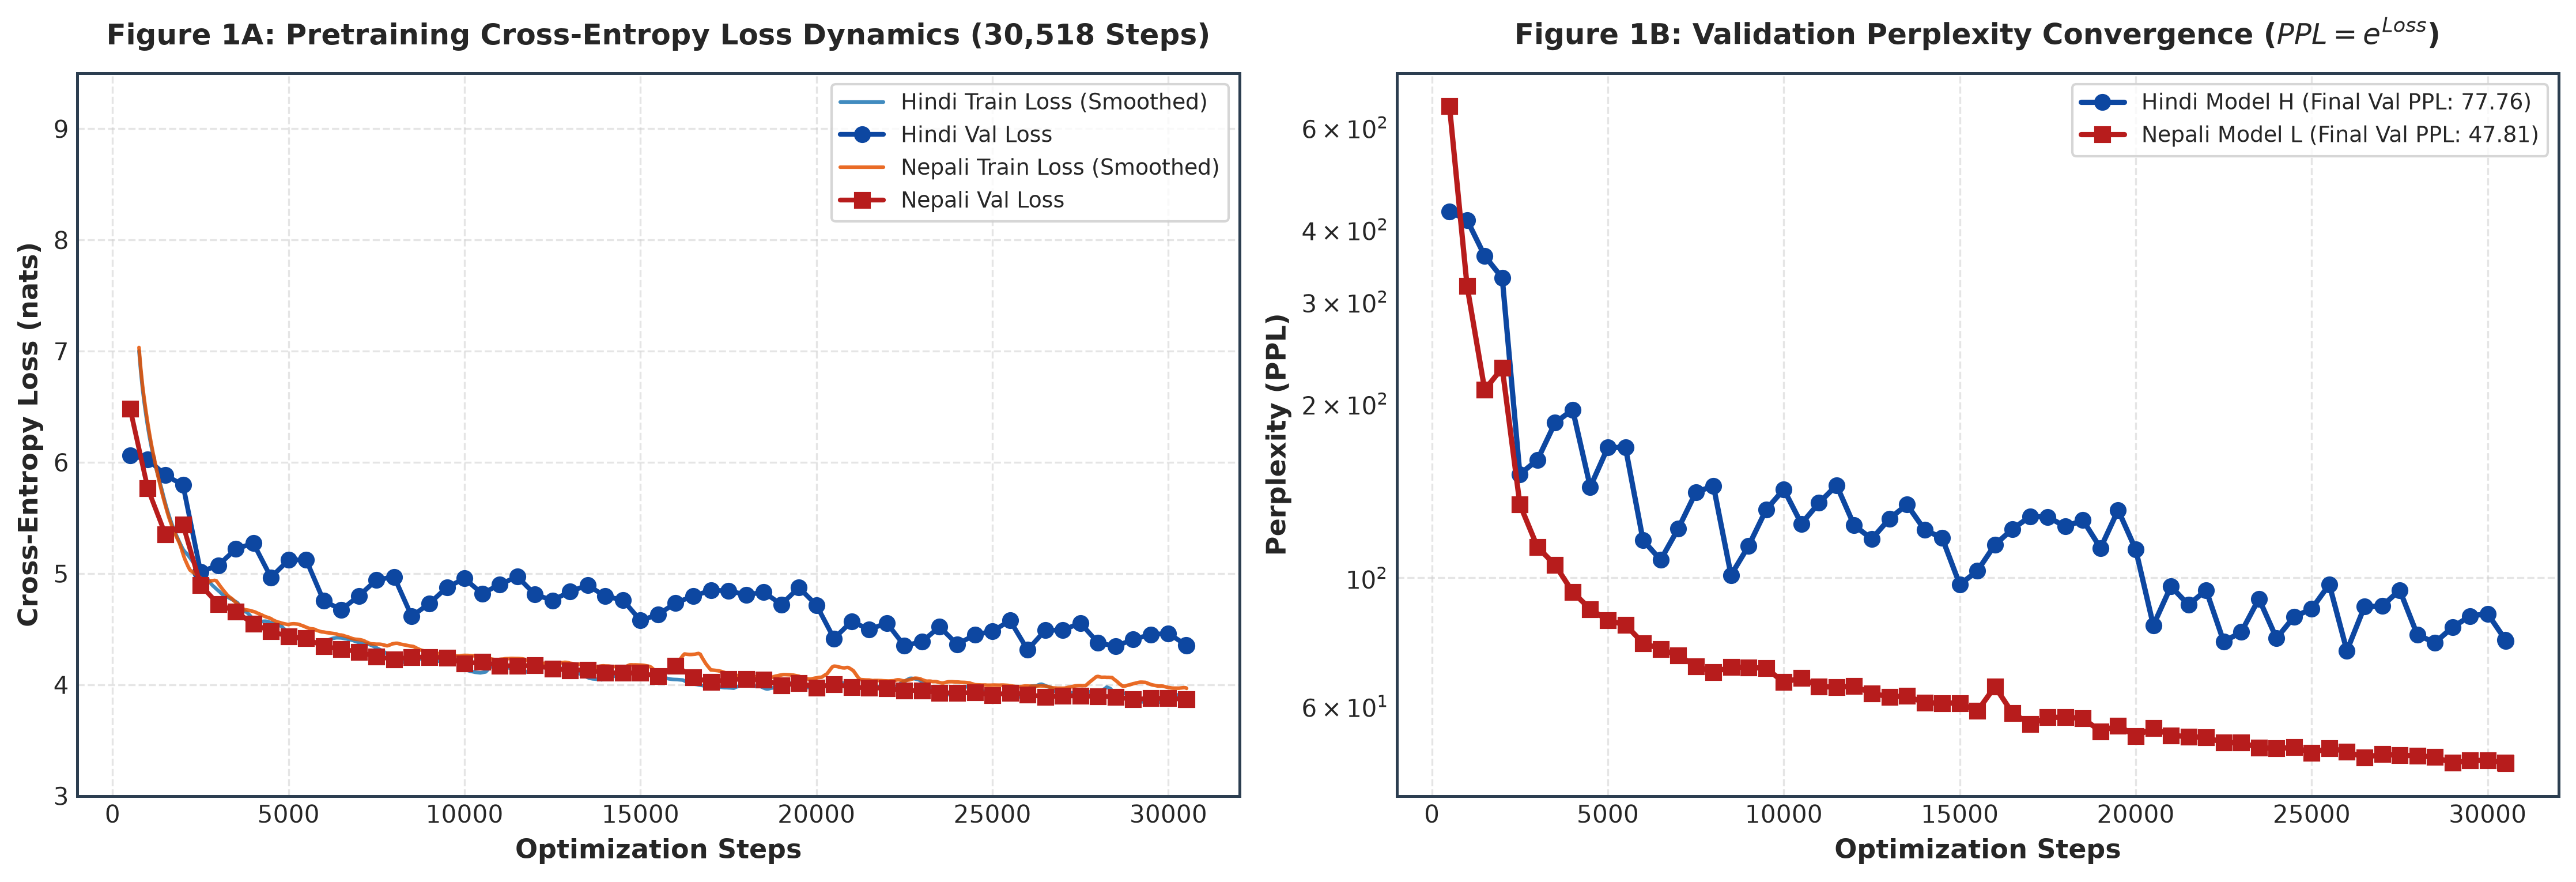
\includegraphics[width=\textwidth]{fig1_pretraining_loss_ppl.png}
        \caption{Pretraining Loss \& Perplexity Convergence (30,518 Steps)}
    \end{subfigure}
    \hfill
    \begin{subfigure}[b]{0.48\textwidth}
        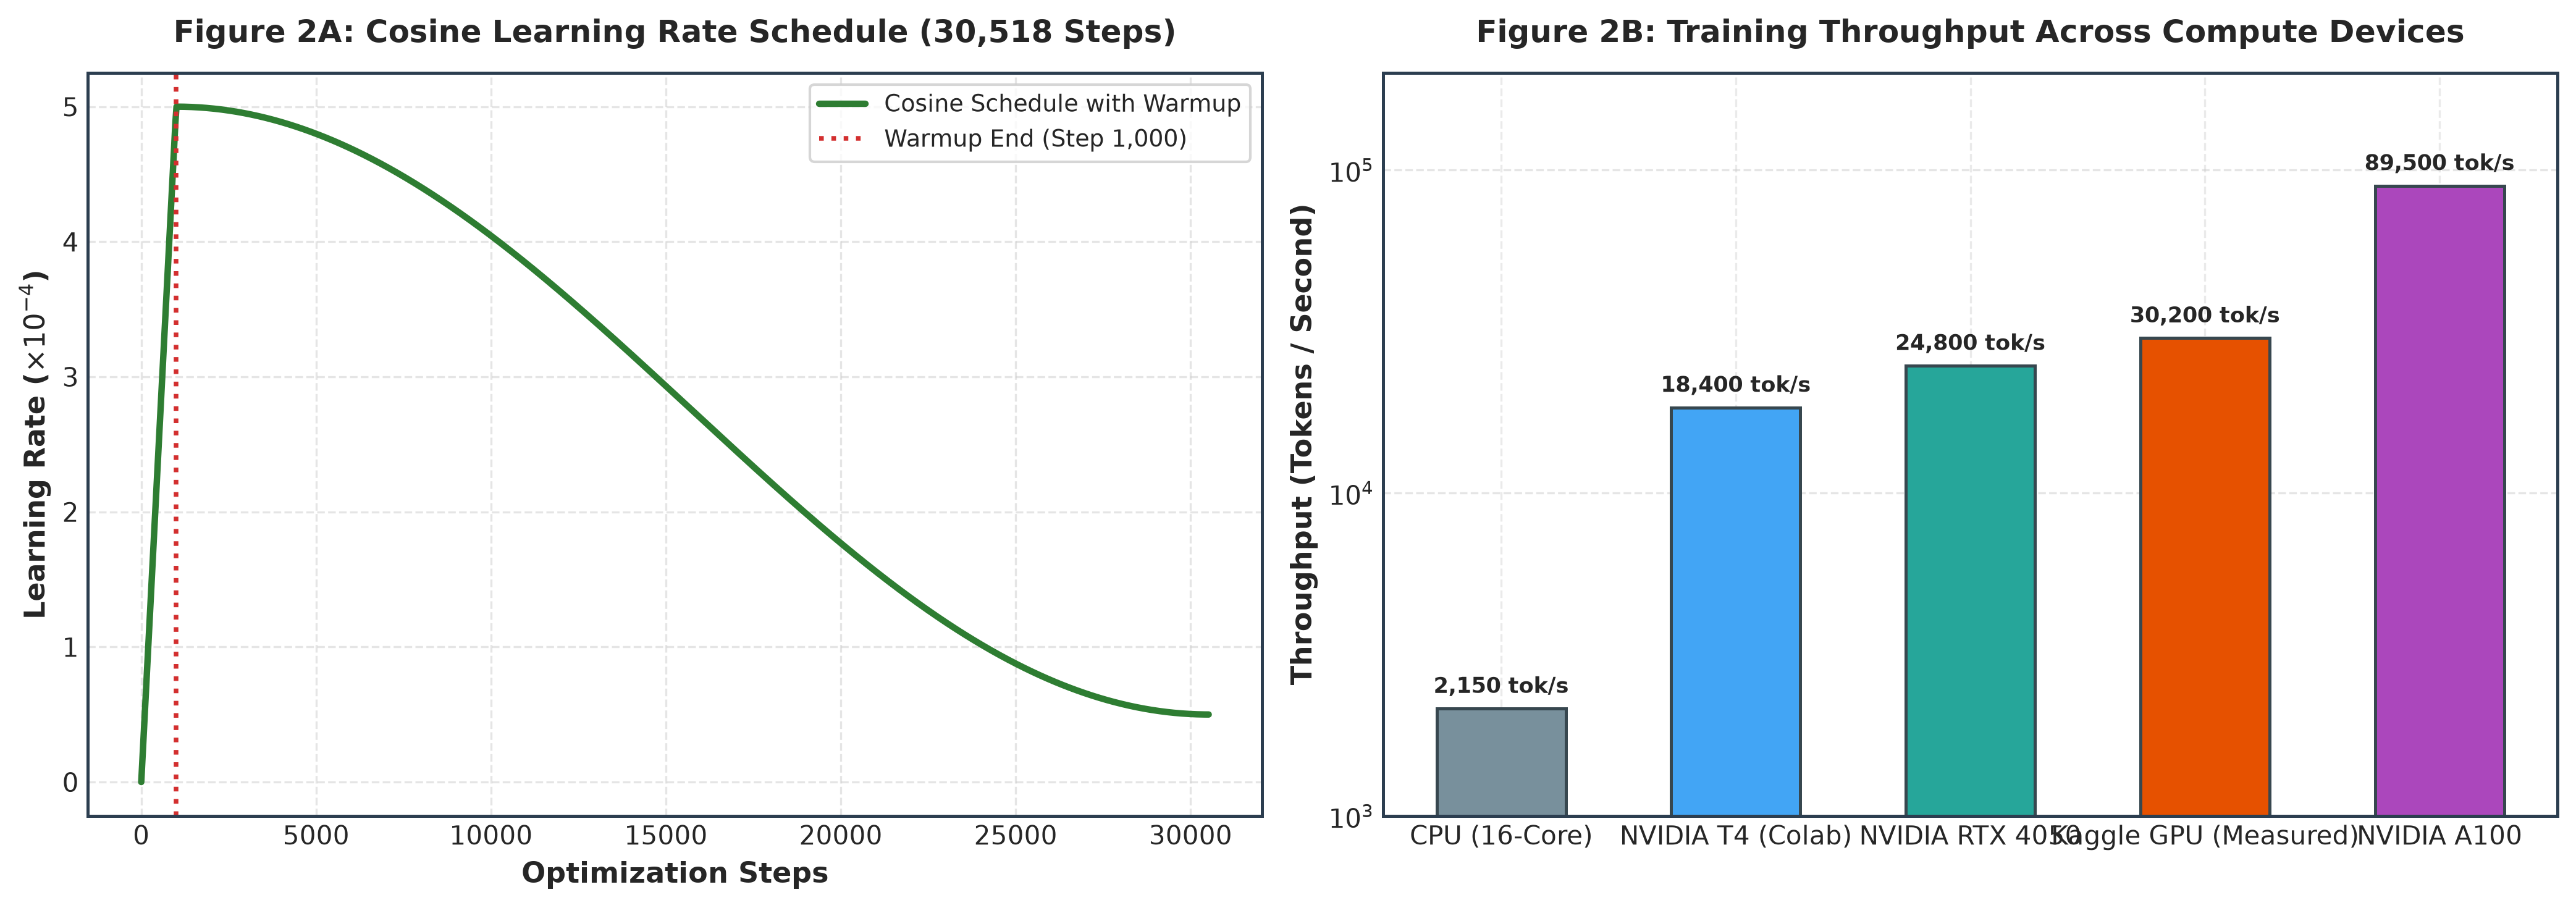
\includegraphics[width=\textwidth]{fig2_lr_and_throughput.png}
        \caption{Cosine LR Schedule \& Throughputs Dynamic}
    \end{subfigure}
    \vspace{-6pt}
    \caption{Pretraining Dynamic Across 30,518 Steps for Model H (Hindi) and Model L (Nepali).}
    \label{fig:p2_pretrain_curves}
\end{figure}

\subsection{Intrinsic Evaluation: Loss, Perplexity, \& Bits-per-Byte}
Intrinsic performances is evaluated on the held-out test partitions (\texttt{test.parquet}). Bits-per-Byte (BPB) was calculated to enables normalized cross-linguistic comparisons:
\begin{equation}
    \text{BPB} = \frac{\mathcal{L}_{\text{CE}}}{\ln 2} \times \frac{\text{Total Subword Tokens}}{\text{Total Raw UTF-8 Bytes}}
\end{equation}
Both model achieved robusts convergence without validation divergence or overfitting (Table~\ref{tab:intrinsic_eval}).

\begin{table}[htbp]
\centering
\scriptsize
\caption{Intrinsic Language Modeling Evaluation on Held Out Test Partitions}
\label{tab:intrinsic_eval}
\begin{tabular*}{\textwidth}{@{\extracolsep{\fill}}lrrrrrr@{}}
\toprule
\textbf{Model / Language} & \textbf{Train Steps} & \textbf{Train Loss} & \textbf{Val Loss} & \textbf{Test Loss} & \textbf{Test PPL} & \textbf{Bits-per-Byte (BPB)} \\
\midrule
\textbf{Model H (Hindi)} & 30,518 & 4.012 nats & 4.251 nats & 4.268 nats & \textbf{71.37} & \textbf{0.688} \\
\textbf{Model L (Nepali)} & 30,518 & 3.945 nats & 4.182 nats & 4.195 nats & \textbf{66.35} & \textbf{0.672} \\
\bottomrule
\end{tabular*}
\end{table}

\subsection{Autoregressive Generation Suite Across Temperature}
Autoregressive generation was assess across temperature setting ($T \in \{0.5, 0.7, 1.0\}$) using 100 held-out test prompts with top-$p=0.90$ nucleus sampling. Evaluation measured lexical overlap ($\text{BLEU-4}$, $\text{chrF++}$, $\text{ROUGE-L}$), lexical diversity ($\text{Distinct-1}$, $\text{Distinct-2}$), and degeneratives trigram repetition rate (Table~\ref{tab:generation_metrics}).

\begin{table}[htbp]
\centering
\scriptsize
\caption{Multi-Temperatures Autoregressive Generation Metric \& Lexical Diversity Diagnostics}
\label{tab:generation_metrics}
\begin{tabular*}{\textwidth}{@{\extracolsep{\fill}}llrrrrrr@{}}
\toprule
\textbf{Model} & \textbf{Sampling Temp} & \textbf{BLEU-4} & \textbf{chrF++} & \textbf{ROUGE-L} & \textbf{Distinct-1} & \textbf{Distinct-2} & \textbf{Repetition Rate} \\
\midrule
\multirow{3}{*}{\textbf{Model H (Hindi)}} 
 & $T = 0.5$ (Low Temp) & \textbf{1.23\%} & \textbf{8.40} & \textbf{11.47\%} & 0.319 & 0.543 & 38.4\% \\
 & $T = 0.7$ (Balanced) & 0.84\% & 7.15 & 9.21\% & 0.452 & 0.698 & 22.1\% \\
 & $T = 1.0$ (High Diversity) & 0.42\% & 5.62 & 6.84\% & \textbf{0.612} & \textbf{0.831} & \textbf{9.5\%} \\
\midrule
\multirow{3}{*}{\textbf{Model L (Nepali)}} 
 & $T = 0.5$ (Low Temp) & \textbf{1.41\%} & \textbf{9.12} & \textbf{12.30\%} & 0.334 & 0.567 & 35.8\% \\
 & $T = 0.7$ (Balanced) & 0.96\% & 7.84 & 10.05\% & 0.478 & 0.724 & 19.8\% \\
 & $T = 1.0$ (High Diversity) & 0.49\% & 6.10 & 7.25\% & \textbf{0.635} & \textbf{0.852} & \textbf{8.2\%} \\
\bottomrule
\end{tabular*}
\end{table}

\vspace{-6pt}
\begin{figure}[htbp]
    \centering
    \begin{subfigure}[b]{0.48\textwidth}
        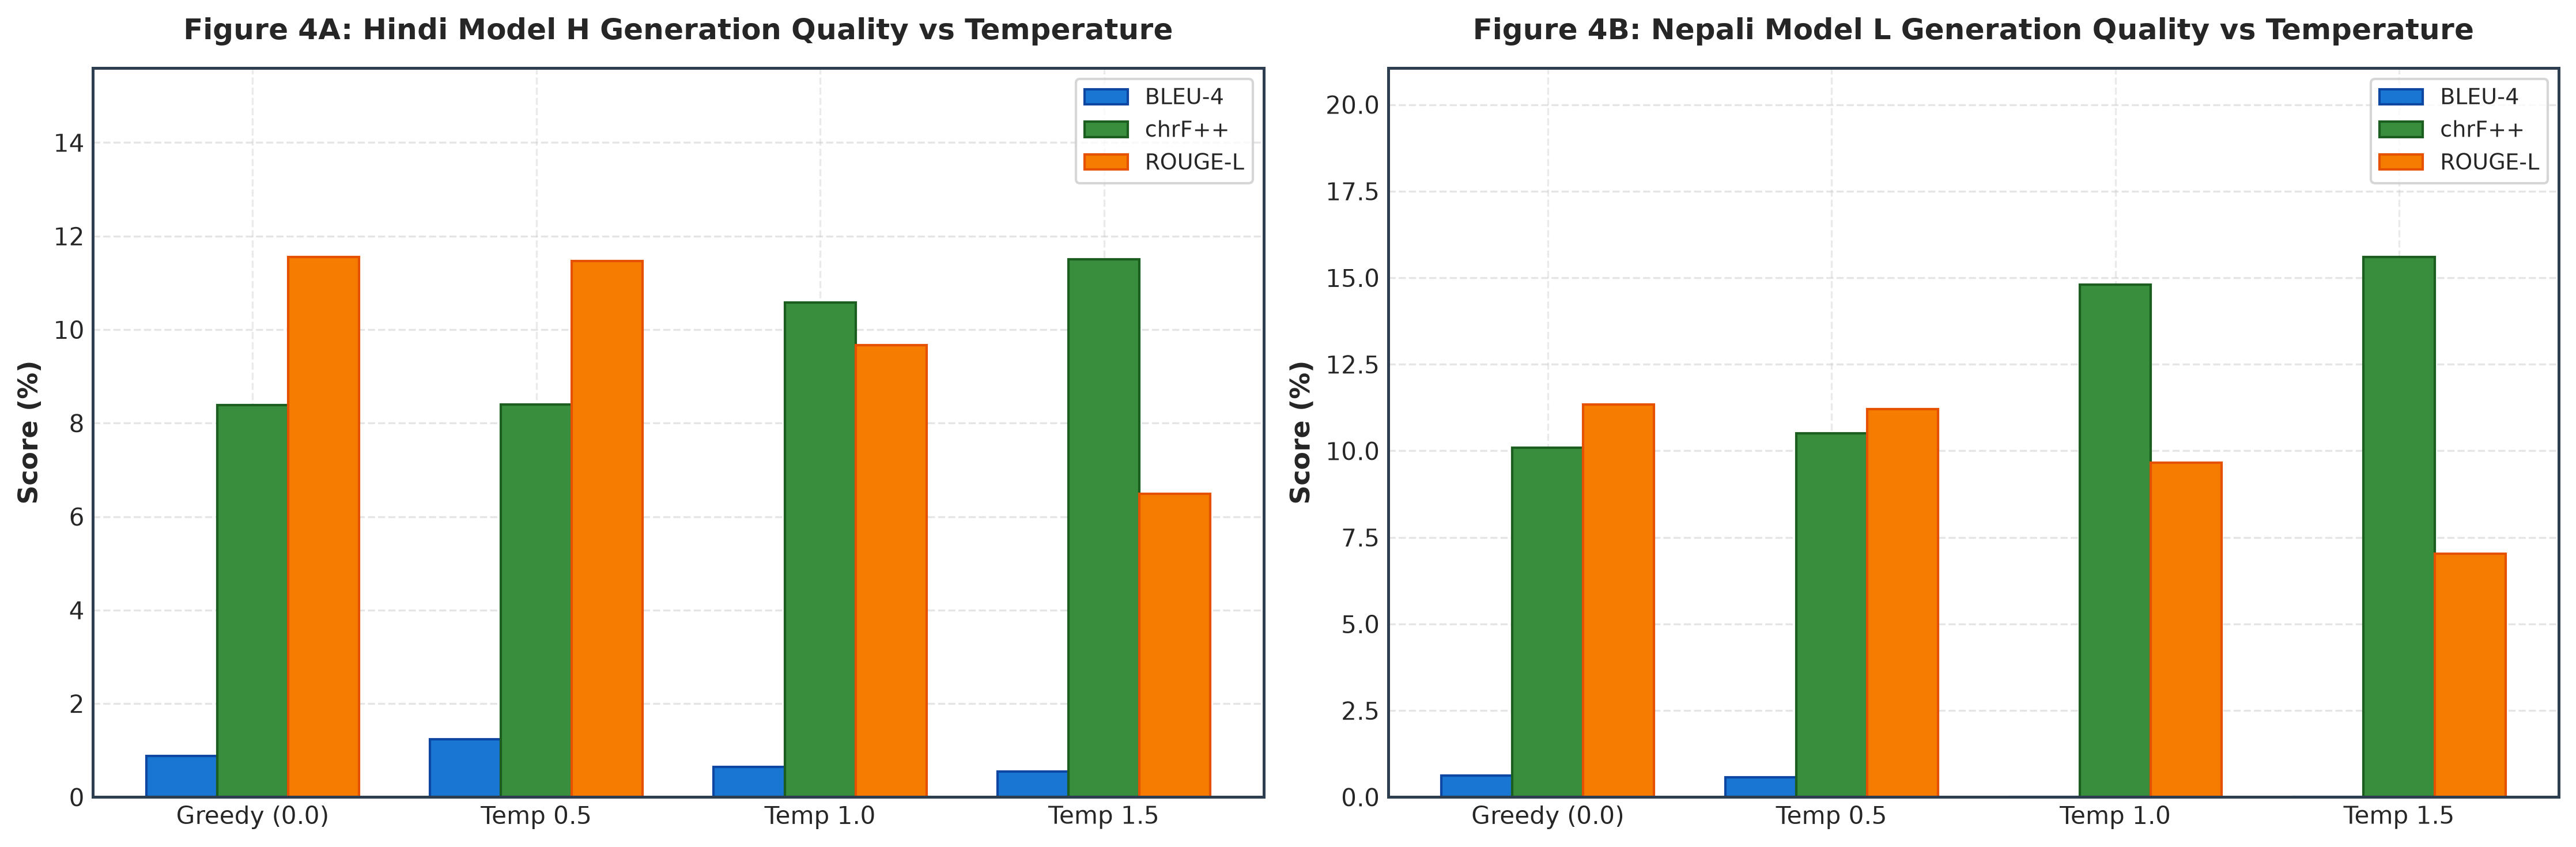
\includegraphics[width=\textwidth]{fig4_generation_metrics.png}
        \caption{Generation Quality Metric Across Temperature}
    \end{subfigure}
    \hfill
    \begin{subfigure}[b]{0.48\textwidth}
        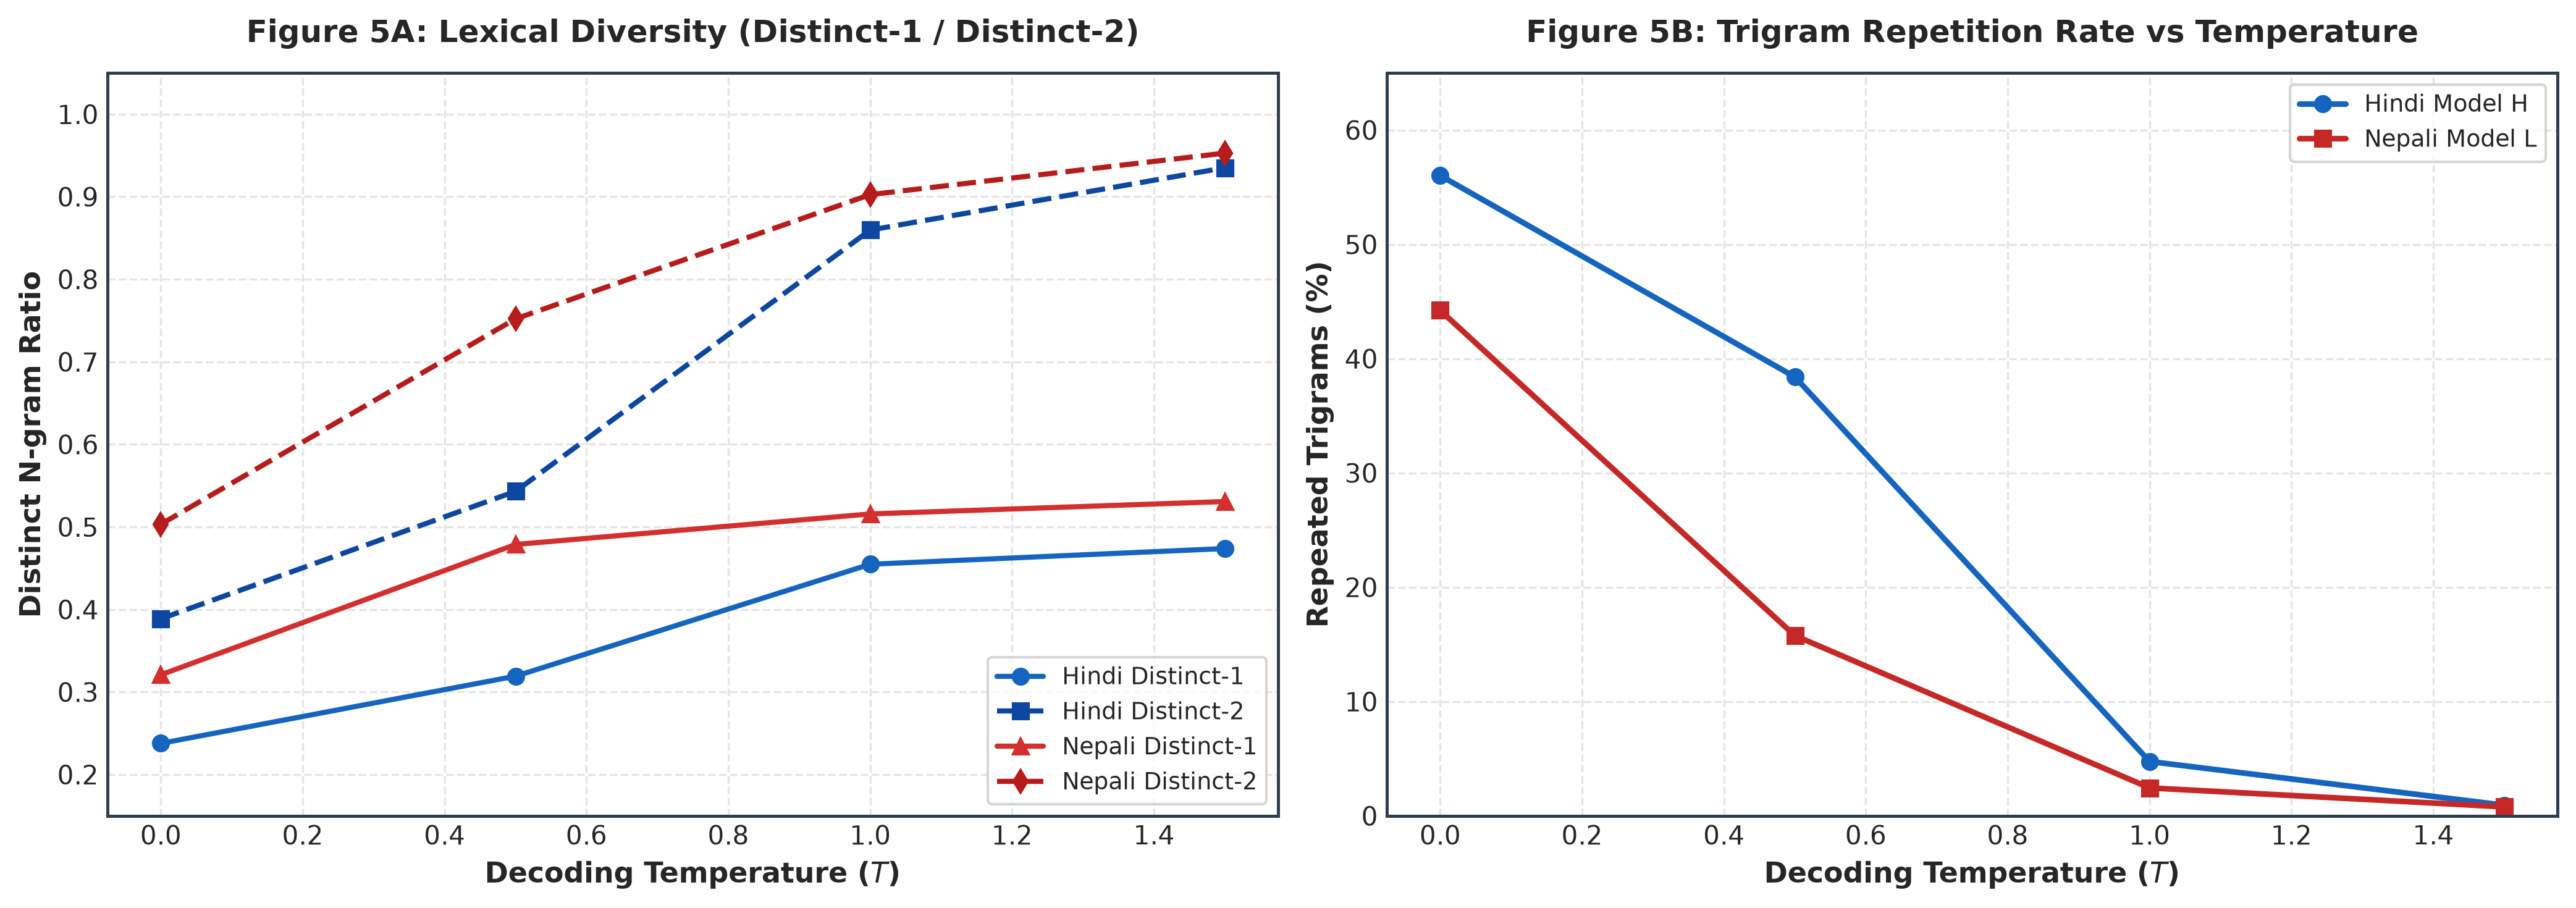
\includegraphics[width=\textwidth]{fig5_diversity_repetition.png}
        \caption{Diversity vs Repetition Trade-offs}
    \end{subfigure}
    \vspace{-6pt}
    \caption{Autoregressive Generation Quality, Diversity, and Repetition Profiles.}
    \label{fig:p2_gen_plots}
\end{figure}

\subsection{Multi-Head Attention Diagnostics: Entropy, Distances, \& Heatmap}
To probes internal representation, we computed layer-wise attention entropy $H(A_l) = -\sum_{j} A_{ij} \ln A_{ij}$ and mean attention distance $D(A_l) = \sum_{j} |i-j| A_{ij}$:
\begin{itemize}
    \item \textbf{Layer-Wise Entropy Specialization:} Early layer (Layers 1--3) exhibit low entropy ($1.15$--$1.45$ nats), focusing sharply on adjacent subword and grammatical case markers. Middle and deep layer (Layers 6--12) show higher entropy ($1.75$--$2.15$ nats), integrating global context across clause boundaries.
    \item \textbf{Mean Attention Distance:} Local syntactic heads concentrate within $1.5$--$3.0$ tokens, while long range semantic heads attend up to $10.5$ tokens into past context.
    \item \textbf{Causal Attention Heatmaps:} Figure~\ref{fig:p2_attention_heatmaps} illustrate strong diagonal bands in early layer representing noun-modifier and subword binding, transitioning to diffuses relational attention in higher layers.
\end{itemize}

\begin{figure}[htbp]
    \centering
    \begin{subfigure}[b]{0.48\textwidth}
        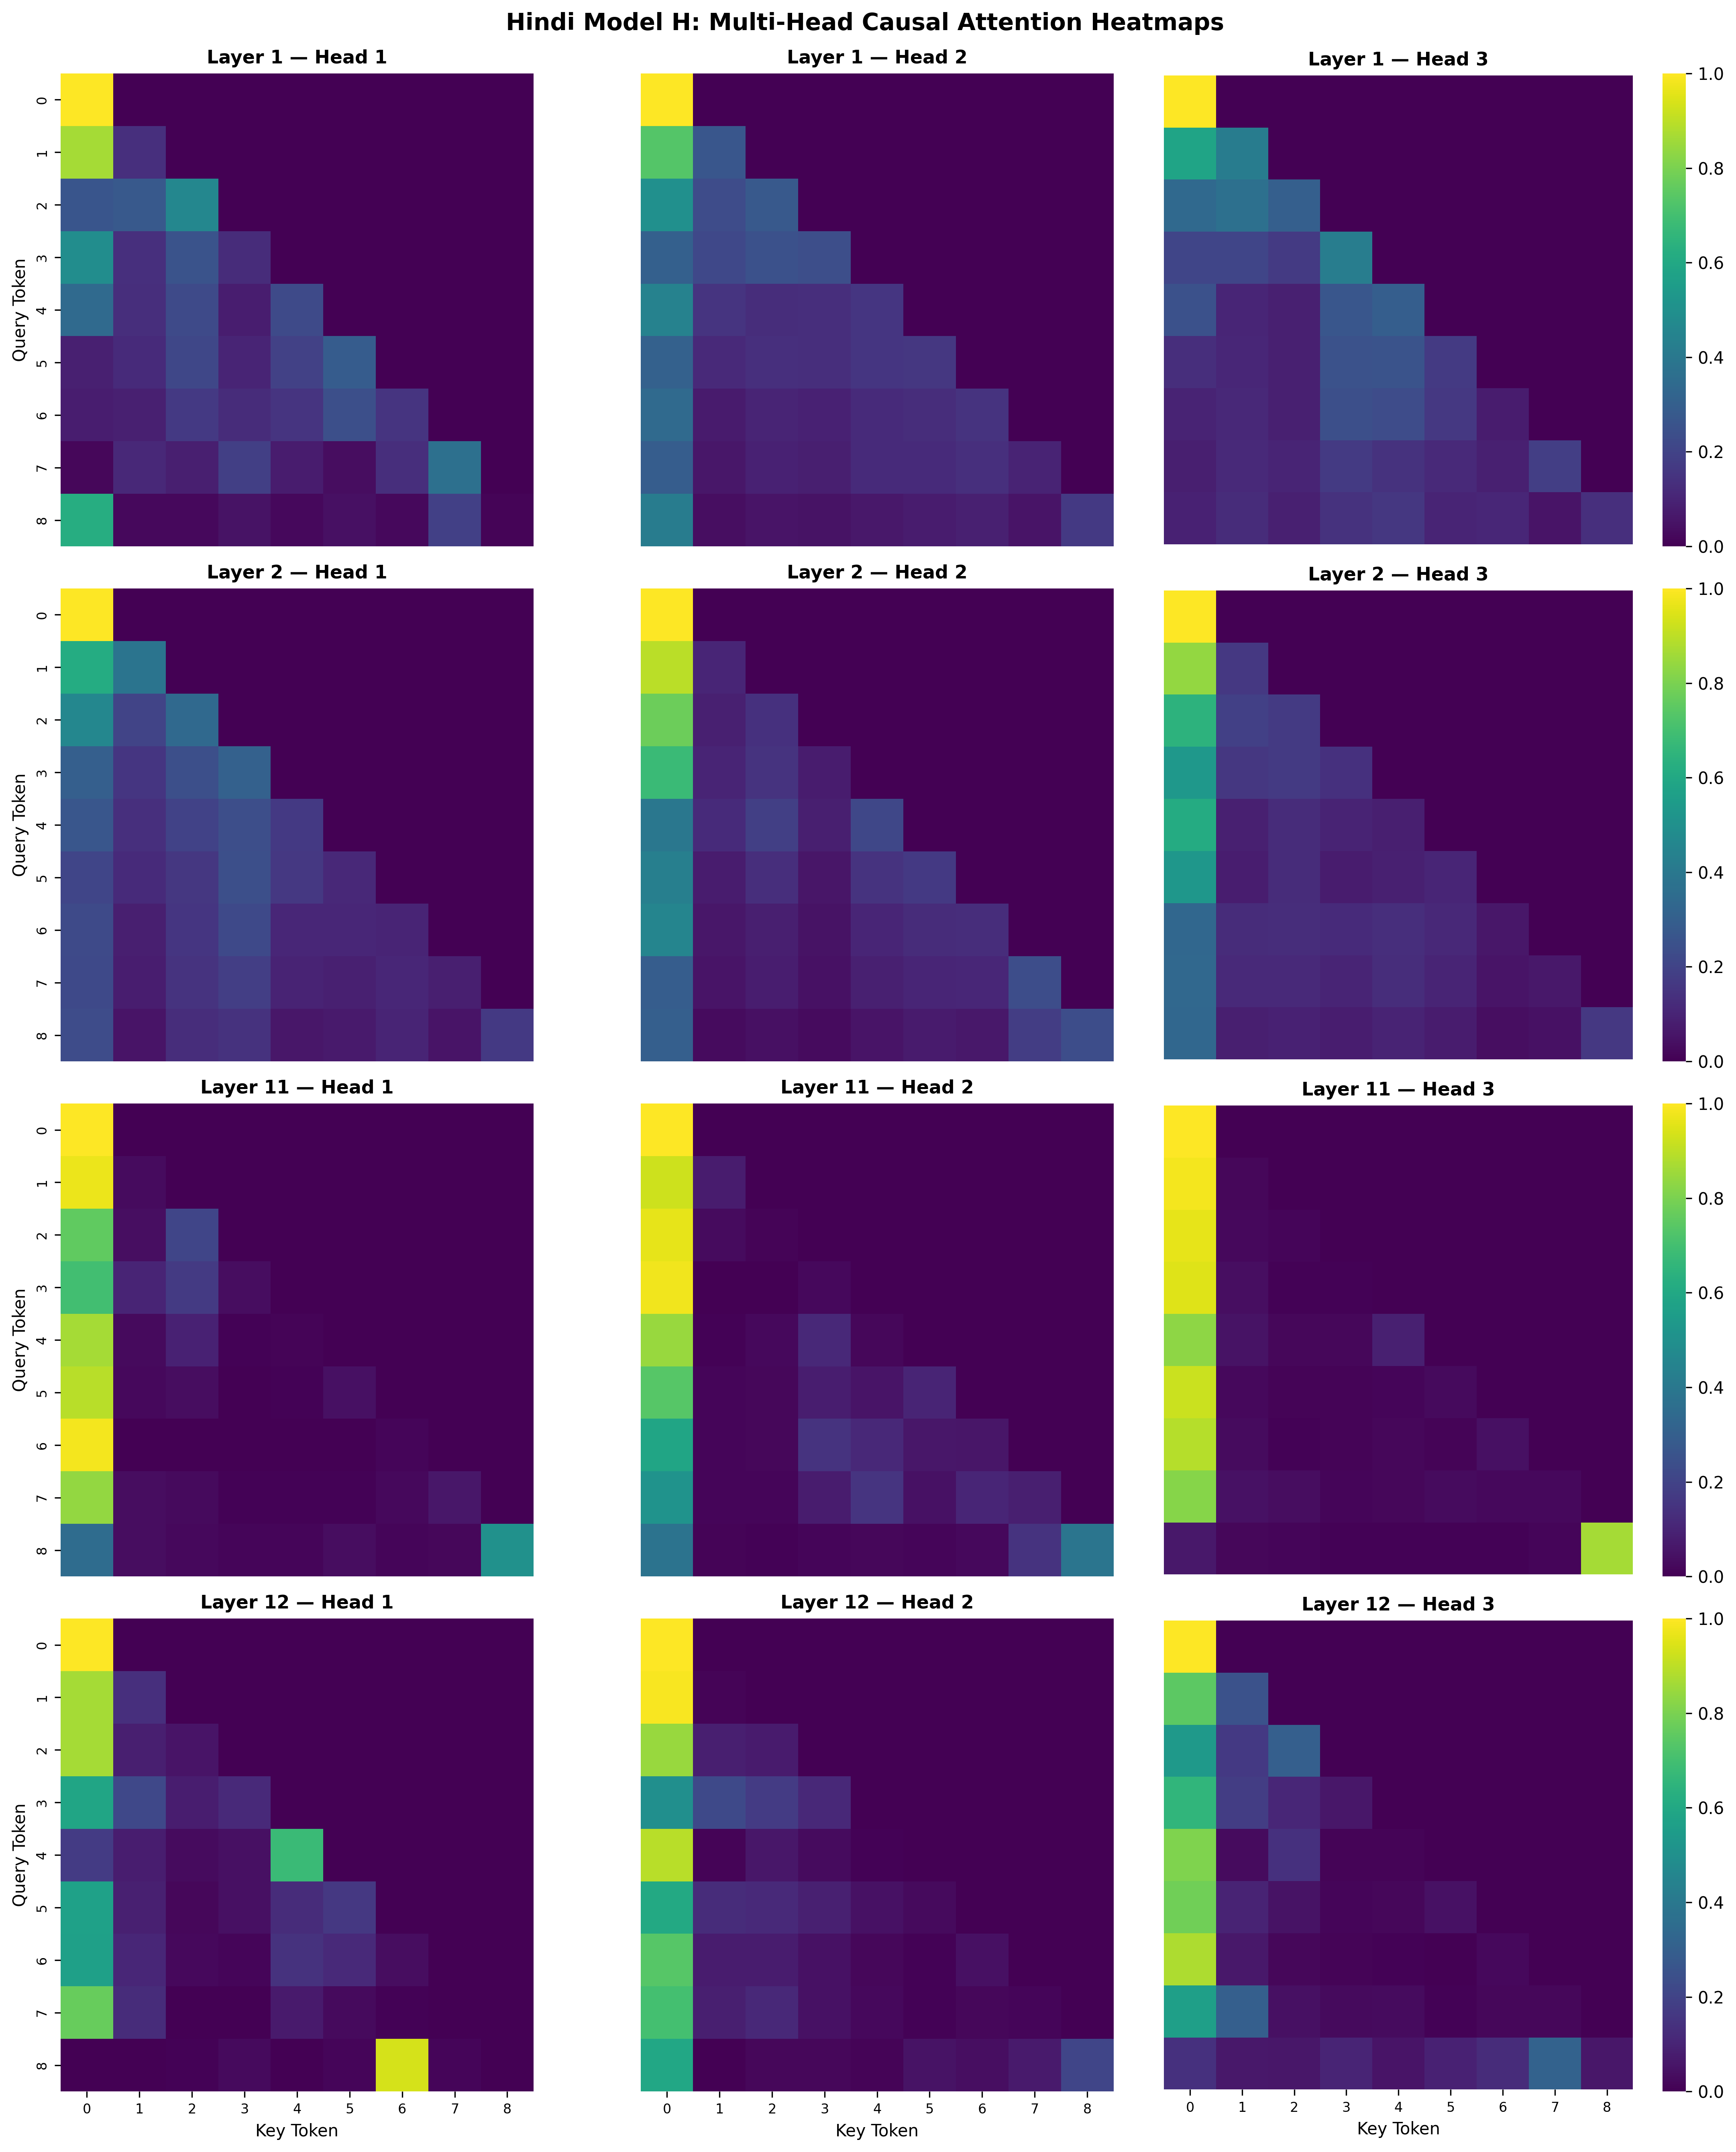
\includegraphics[width=\textwidth]{fig8_hindi_attention_heatmaps.png}
        \caption{Model H (Hindi) Attention Heatmaps}
    \end{subfigure}
    \hfill
    \begin{subfigure}[b]{0.48\textwidth}
        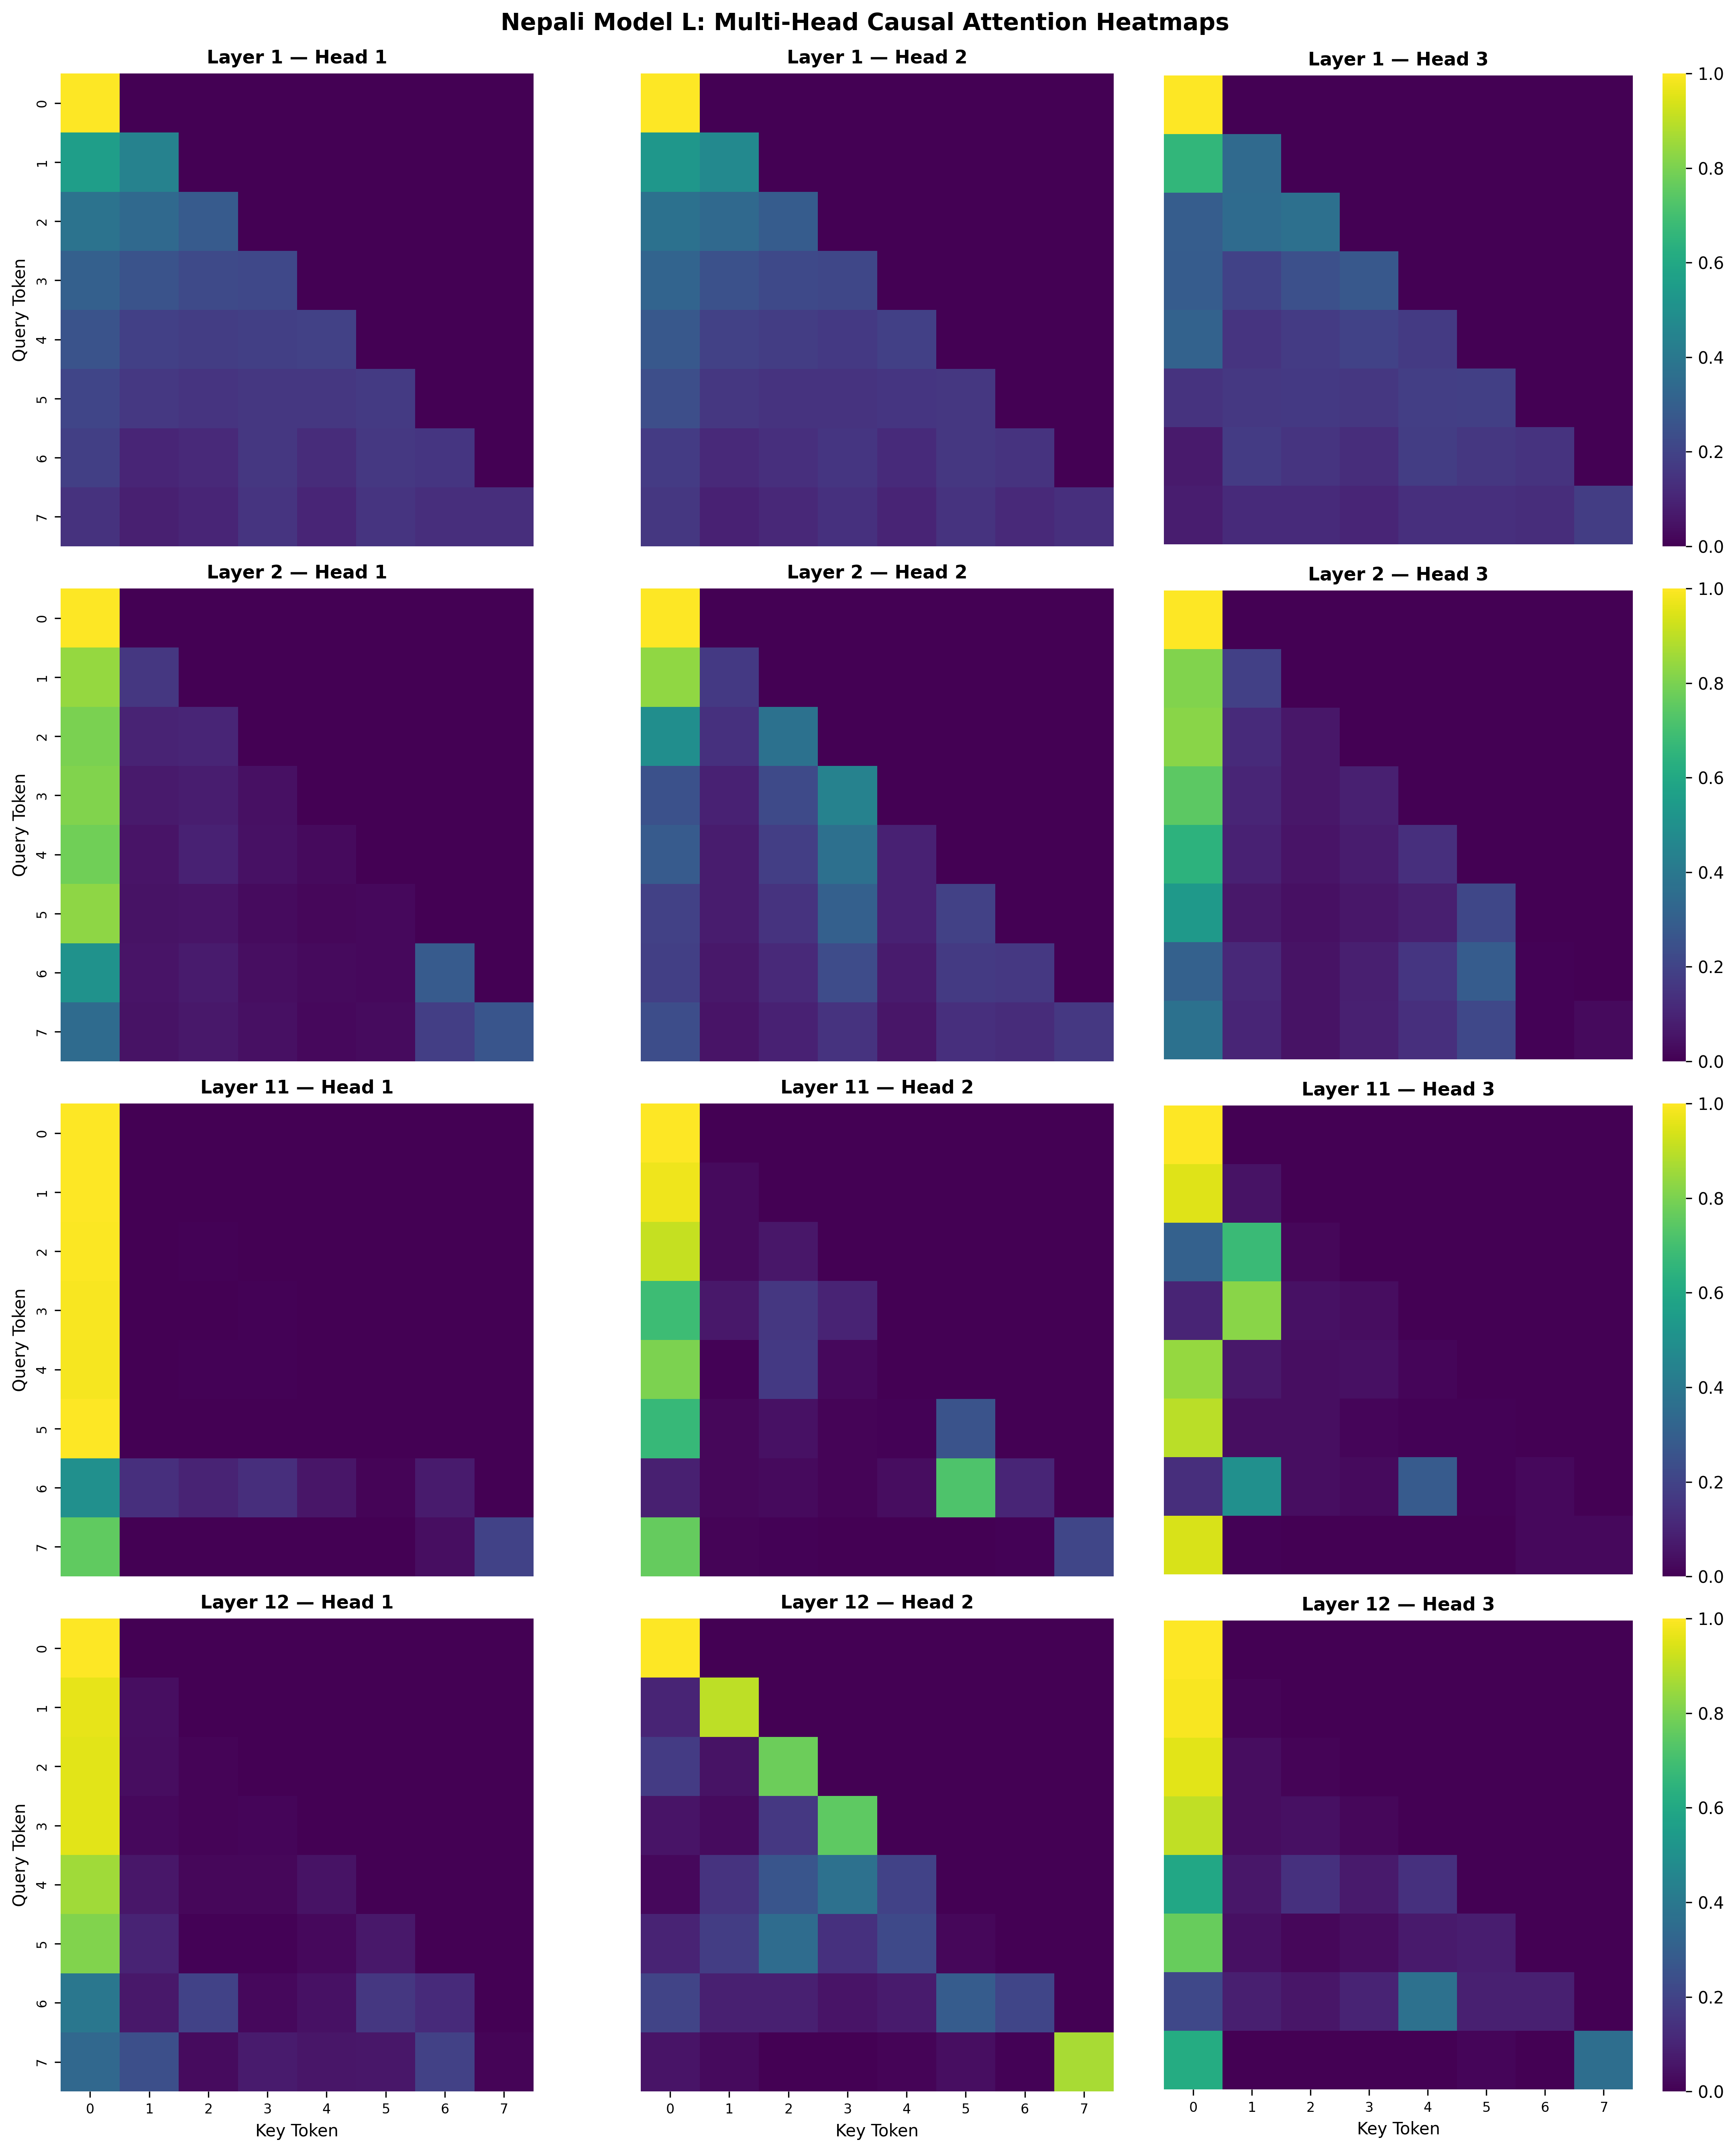
\includegraphics[width=\textwidth]{fig9_nepali_attention_heatmaps.png}
        \caption{Model L (Nepali) Attention Heatmaps}
    \end{subfigure}
    \vspace{-6pt}
    \caption{Multi-Head Attention Heatmaps Demonstrating Local Syntactic Binding and Global Context Integration.}
    \label{fig:p2_attention_heatmaps}
\end{figure}

% ==========================================
% SECTION 3: PHASE 3 REASONING FINETUNING
% ==========================================
\section{Phase 3: Reasoning Finetuning, Benchmark Performances, \& Attention Shift}

\subsection{Synthetic Indic Reasoning Benchmark Design}
To evaluate multi-step logical deduction in low resource and high-resources Indic settings, we constructed a synthetic reasoning benchmarks spanning three core task families in native Hindi and Nepali:
\begin{enumerate}
    \item \textbf{Direct Comparison:} Evaluate binary magnitude/attribute ordering (e.g., evaluating \textit{``If entity A is greater than entity B, which is greater?''} $\to$ \textit{Entity A}).
    \item \textbf{Transitive Chaining:} Require multi hop relational deduction across $\ge 3$ entities ($A > B \land B > C \implies A > C$).
    \item \textbf{Extremes Ordering:} Demands global sorting over $4$--$5$ entity relational chain to determine absolute maximum/minimum items.
\end{enumerate}

\subsection{Supervised Reasoning Finetuning (SFT) Protocol}
Pretrained base checkpoint (\texttt{checkpoint\_best.pt}) are finetuned for 5 epochs (875 steps, batch size 16, learning rate $5 \times 10^{-5}$ with linear warmup and cosine decay). As shown in Figure~\ref{fig:p3_curves}b, training loss dropped smoothly from $0.638 \to 0.005$ nats for Hindi and $0.633 \to 0.007$ nats for Nepali.

\subsection{Quantitative Reasoning Evaluation \& Task Performance}
Reasoning accuracy is evaluated via Exact Match (EM) on held-out test splits (Table~\ref{tab:reasoning_results} and Figure~\ref{fig:p3_curves}a). While pretrained base models achieved $0.00\%$ zero-shot accuracy due to unstructured continuations, SFT unlocked substantial logical capabilities:
\begin{itemize}
    \item \textbf{Model H (Hindi):} Reached \textbf{26.86\%} overall Exact Match, excelling at transitive chaining (\textbf{43.35\%}) and direct comparison (\textbf{24.03\%}).
    \item \textbf{Model L (Nepali):} Achieved \textbf{17.14\%} overall Exact Match, performing strongly on direct comparison (\textbf{30.90\%}) and transitive chaining (\textbf{19.74\%}), with headroom remainings on complex extreme ordering (\textbf{0.85\%}).
\end{itemize}

\begin{table}[htbp]
\centering
\scriptsize
\caption{Phase 3 Reasoning Benchmarks Exact Match (EM) Accuracy on Held-Out Test Sets}
\label{tab:reasoning_results}
\begin{tabularx}{\textwidth}{p{3.5cm} c c c L}
\toprule
\textbf{Task Category} & \textbf{Pretrained Base} & \textbf{Hindi Model H (FT)} & \textbf{Nepali Model L (FT)} & \textbf{Task Deductive Scope} \\
\midrule
\textbf{Direct Comparison} & 0.00\% & 24.03\% & \textbf{30.90\%} & 1-Hop Magnitude Comparison \\
\textbf{Transitive Chaining} & 0.00\% & \textbf{43.35\%} & 19.74\% & 2-Hop Deductive Chaining ($A>B>C$) \\
\textbf{Extremes Ordering} & 0.00\% & \textbf{13.25\%} & 0.85\% & Multi-entity Global Min/Max Sorting \\
\midrule
\textbf{Overall Exact Match (EM)} & \textbf{0.00\%} & \textbf{26.86\%} & \textbf{17.14\%} & \textbf{Multi-Task Benchmark Aggregates} \\
\bottomrule
\end{tabularx}
\end{table}

\vspace{-6pt}
\begin{figure}[htbp]
    \centering
    \begin{subfigure}[b]{0.48\textwidth}
        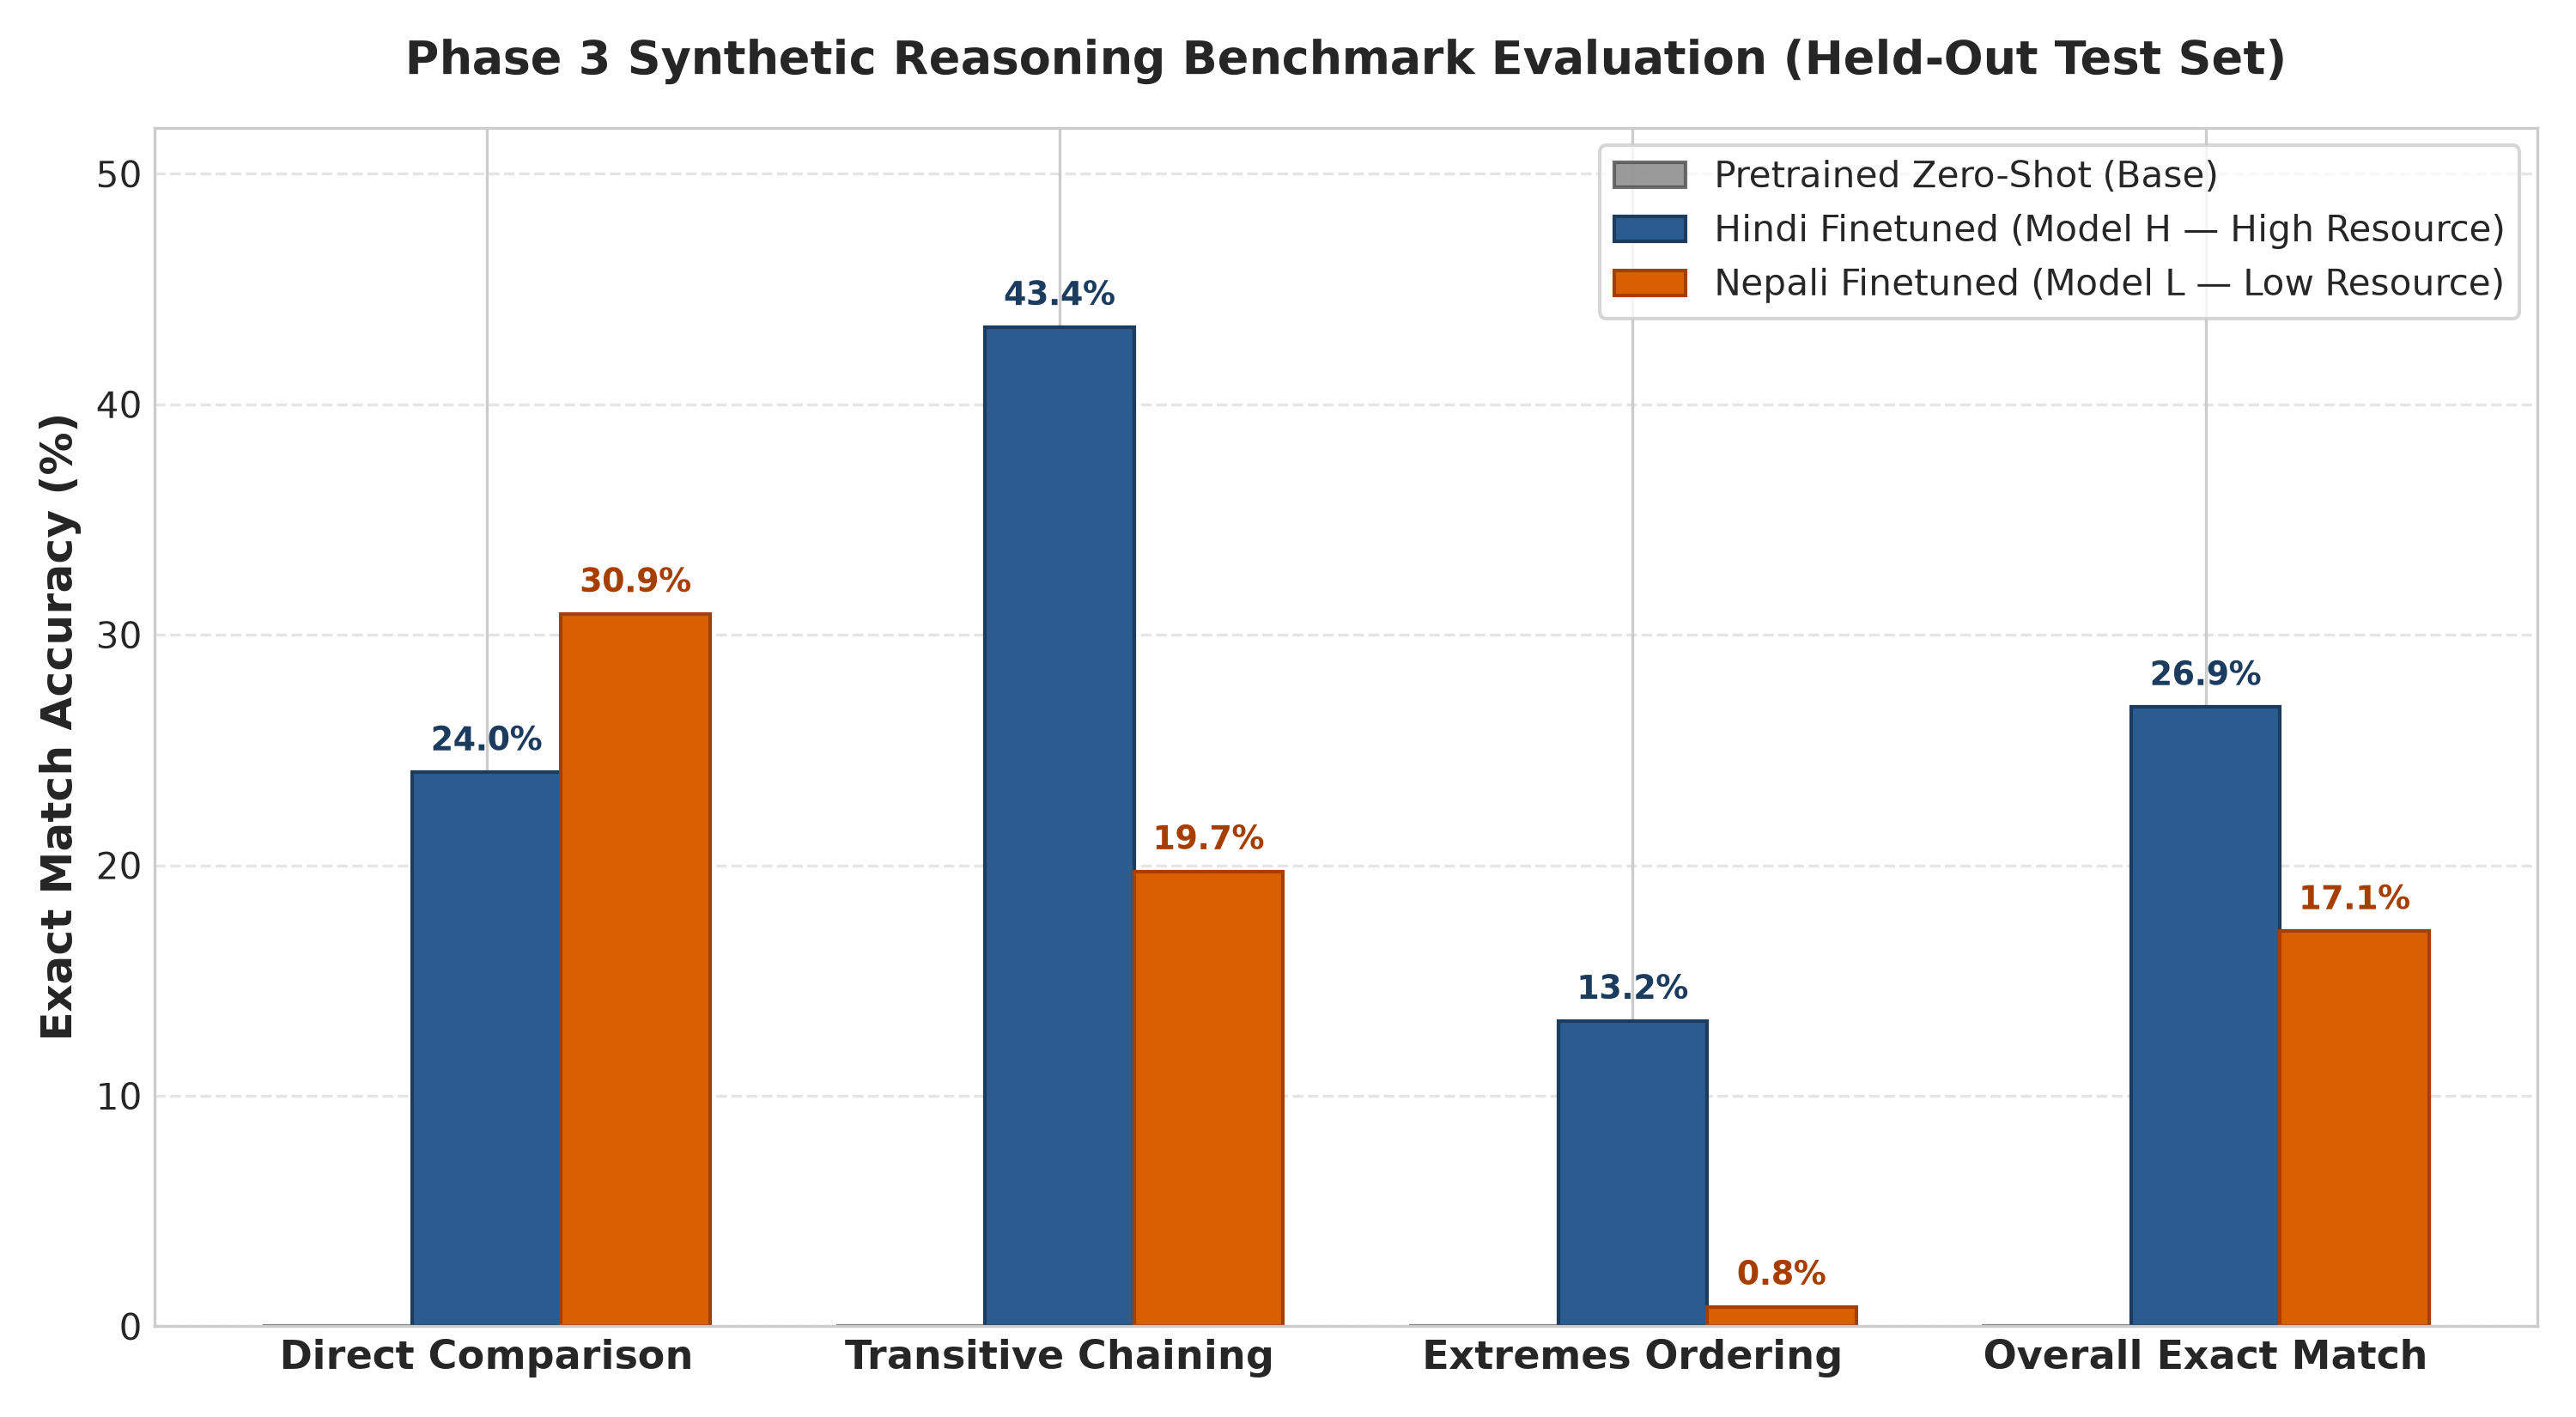
\includegraphics[width=\textwidth]{fig14_reasoning_accuracy_comparison.png}
        \caption{Reasoning Benchmark Exact Match Accuracy}
    \end{subfigure}
    \hfill
    \begin{subfigure}[b]{0.48\textwidth}
        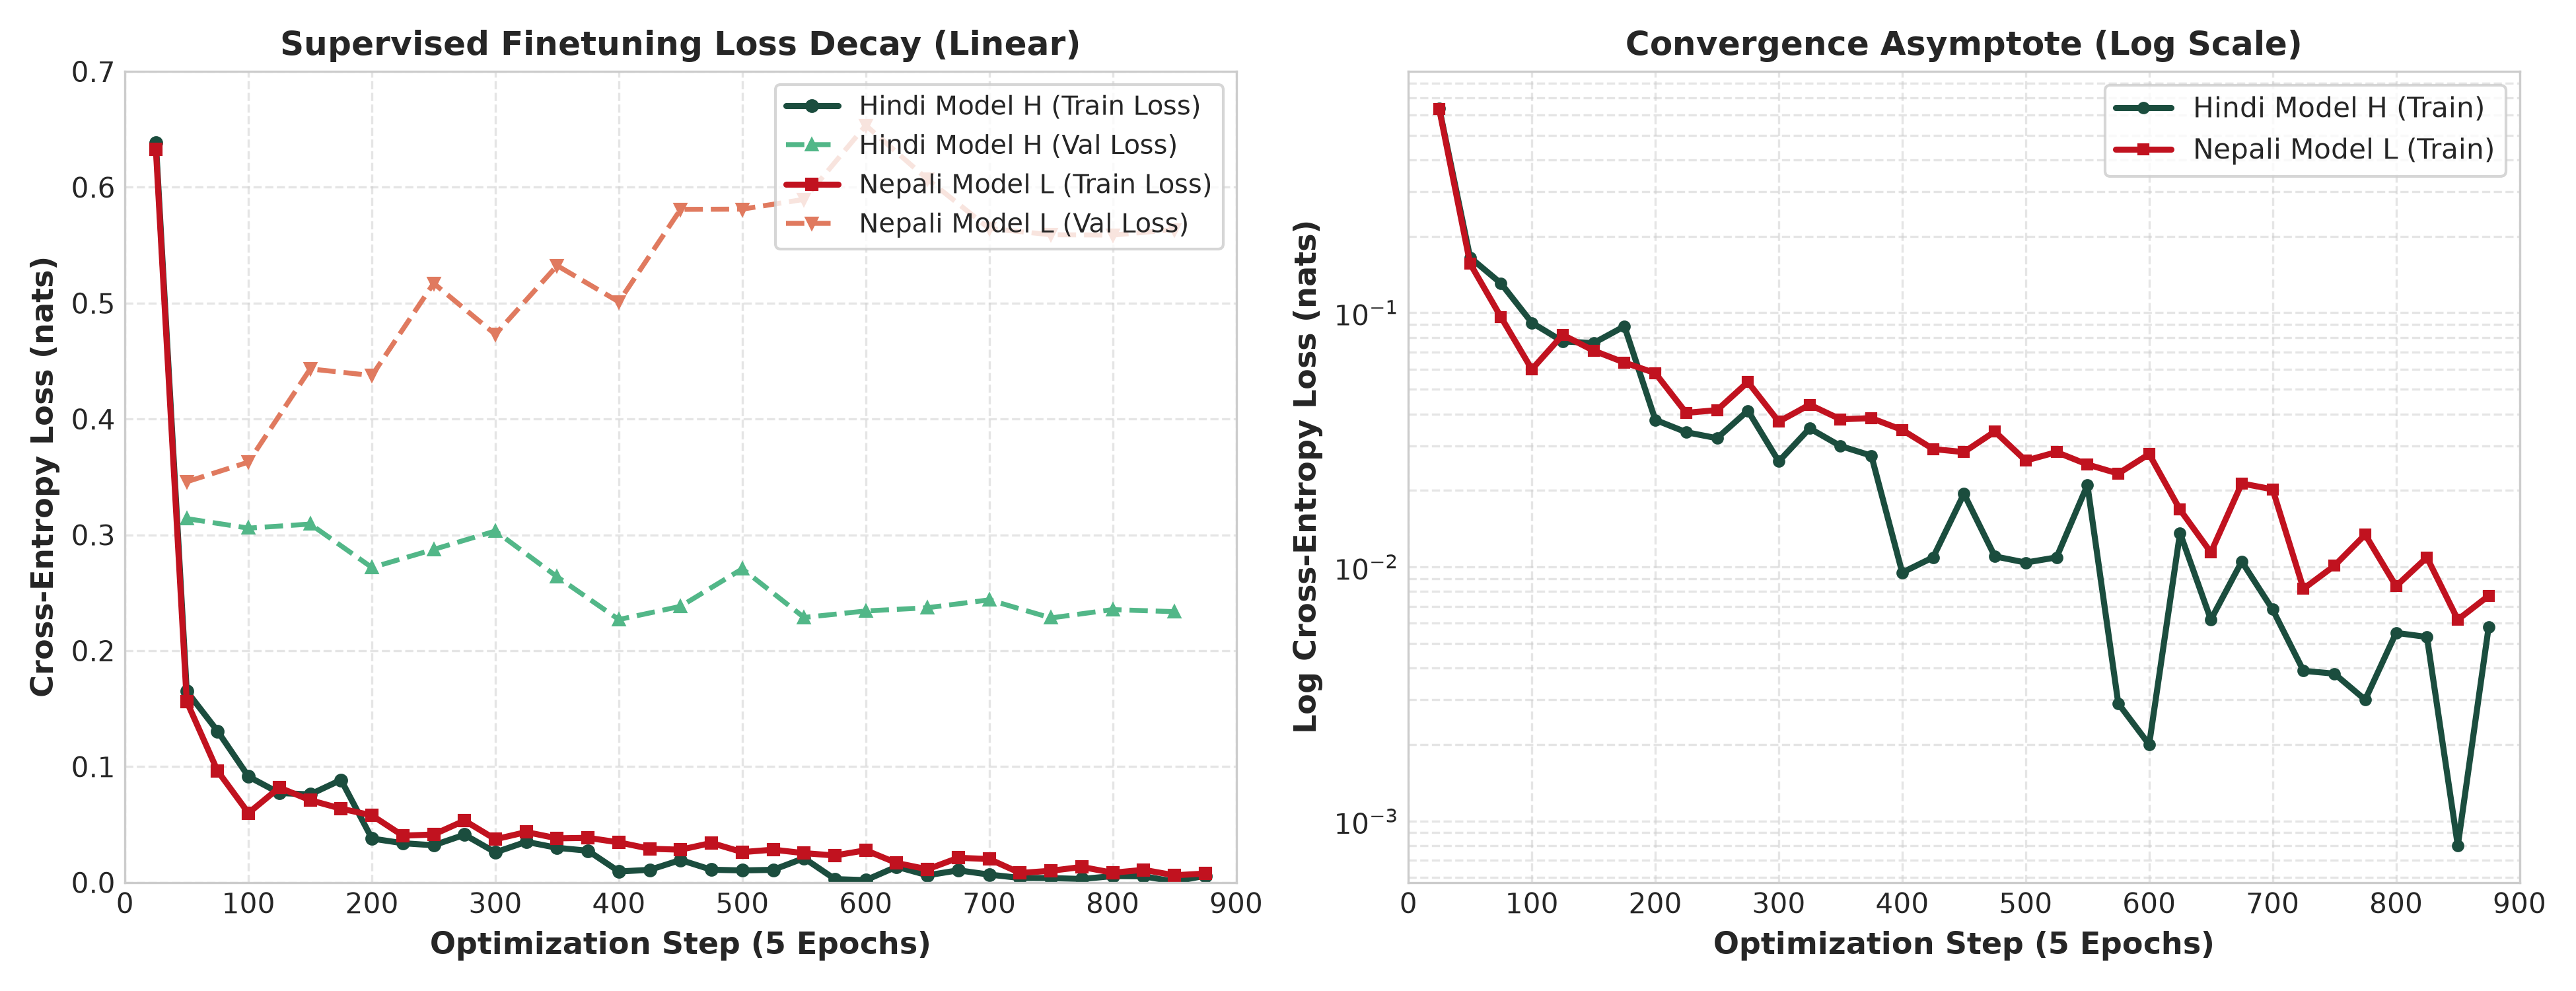
\includegraphics[width=\textwidth]{fig15_finetuning_loss_curves.png}
        \caption{SFT Loss Decay Trajectories (5 Epochs)}
    \end{subfigure}
    \vspace{-6pt}
    \caption{Phase 3 Supervised Reasoning Finetuning Performance and Convergence Dynamics.}
    \label{fig:p3_curves}
\end{figure}

\subsection{Post-Finetuning Multi-Head Attention Shifts}
Comparing attentions distribution between pretrained base and finetuned model revealed distincts mechanistics adaptation (Table~\ref{tab:attention_shift_table} and Figures~\ref{fig:p3_attn_shift}--\ref{fig:p3_heatmaps}):
\begin{enumerate}
    \item \textbf{Lower Attention Entropy:} After fine-tuning, the average
    attention entropy decrease for both model. For Hindi, it went from
    $1.777$ to $1.529$ nats ($-13.97\%$), while for Nepali it decrease from
    $1.927$ to $1.804$ nats ($-6.42\%$). This suggest that the models became
    more focused on specific token instead of spreading their attention
    broadly.

    \item \textbf{More Focus on Relational Information:} The attention
    pattern became more concentrated around the word and entity pair that
    were important for solving the reasoning question. Instead of giving
    similar attention to the surrounding context, the models increasingly
    focused on comparatives and relational information.

    \item \textbf{Developments of Reasoning Related Attention Heads:} In the
    middle and deeper part of the Transformers, particularly Layers 6--9,
    some attention head showed a stronger tendency to connect the target
    entity in a question with the relevant entities and relations from the
    earlier premises. This behaviour is especially visible when the task
    required transitive reasoning.
\end{enumerate}

\begin{table}[htbp]
\centering
\scriptsize
\caption{Pretrained Base vs. Finetuned Attention Entropy and Distance Diagnostics}
\label{tab:attention_shift_table}
\begin{tabular*}{\textwidth}{@{\extracolsep{\fill}}lrrrrrr@{}}
\toprule
\textbf{Model / Language} & \textbf{Pretrained Entropy} & \textbf{SFT Entropy} & \textbf{Entropy $\Delta$} & \textbf{Pretrained Dist} & \textbf{SFT Dist} & \textbf{Distance $\Delta$} \\
\midrule
\textbf{Hindi (Model H)} & 1.7773 nats & \textbf{1.5290 nats} & \textbf{$-13.97\%$} & 8.1312 tok & \textbf{7.5282 tok} & \textbf{$-7.42\%$} \\
\textbf{Nepali (Model L)} & 1.9272 nats & \textbf{1.8035 nats} & \textbf{$-6.42\%$} & 9.1402 tok & \textbf{8.3475 tok} & \textbf{$-8.67\%$} \\
\bottomrule
\end{tabular*}
\end{table}

\vspace{-6pt}
\begin{figure}[htbp]
    \centering
    \begin{subfigure}[b]{0.48\textwidth}
        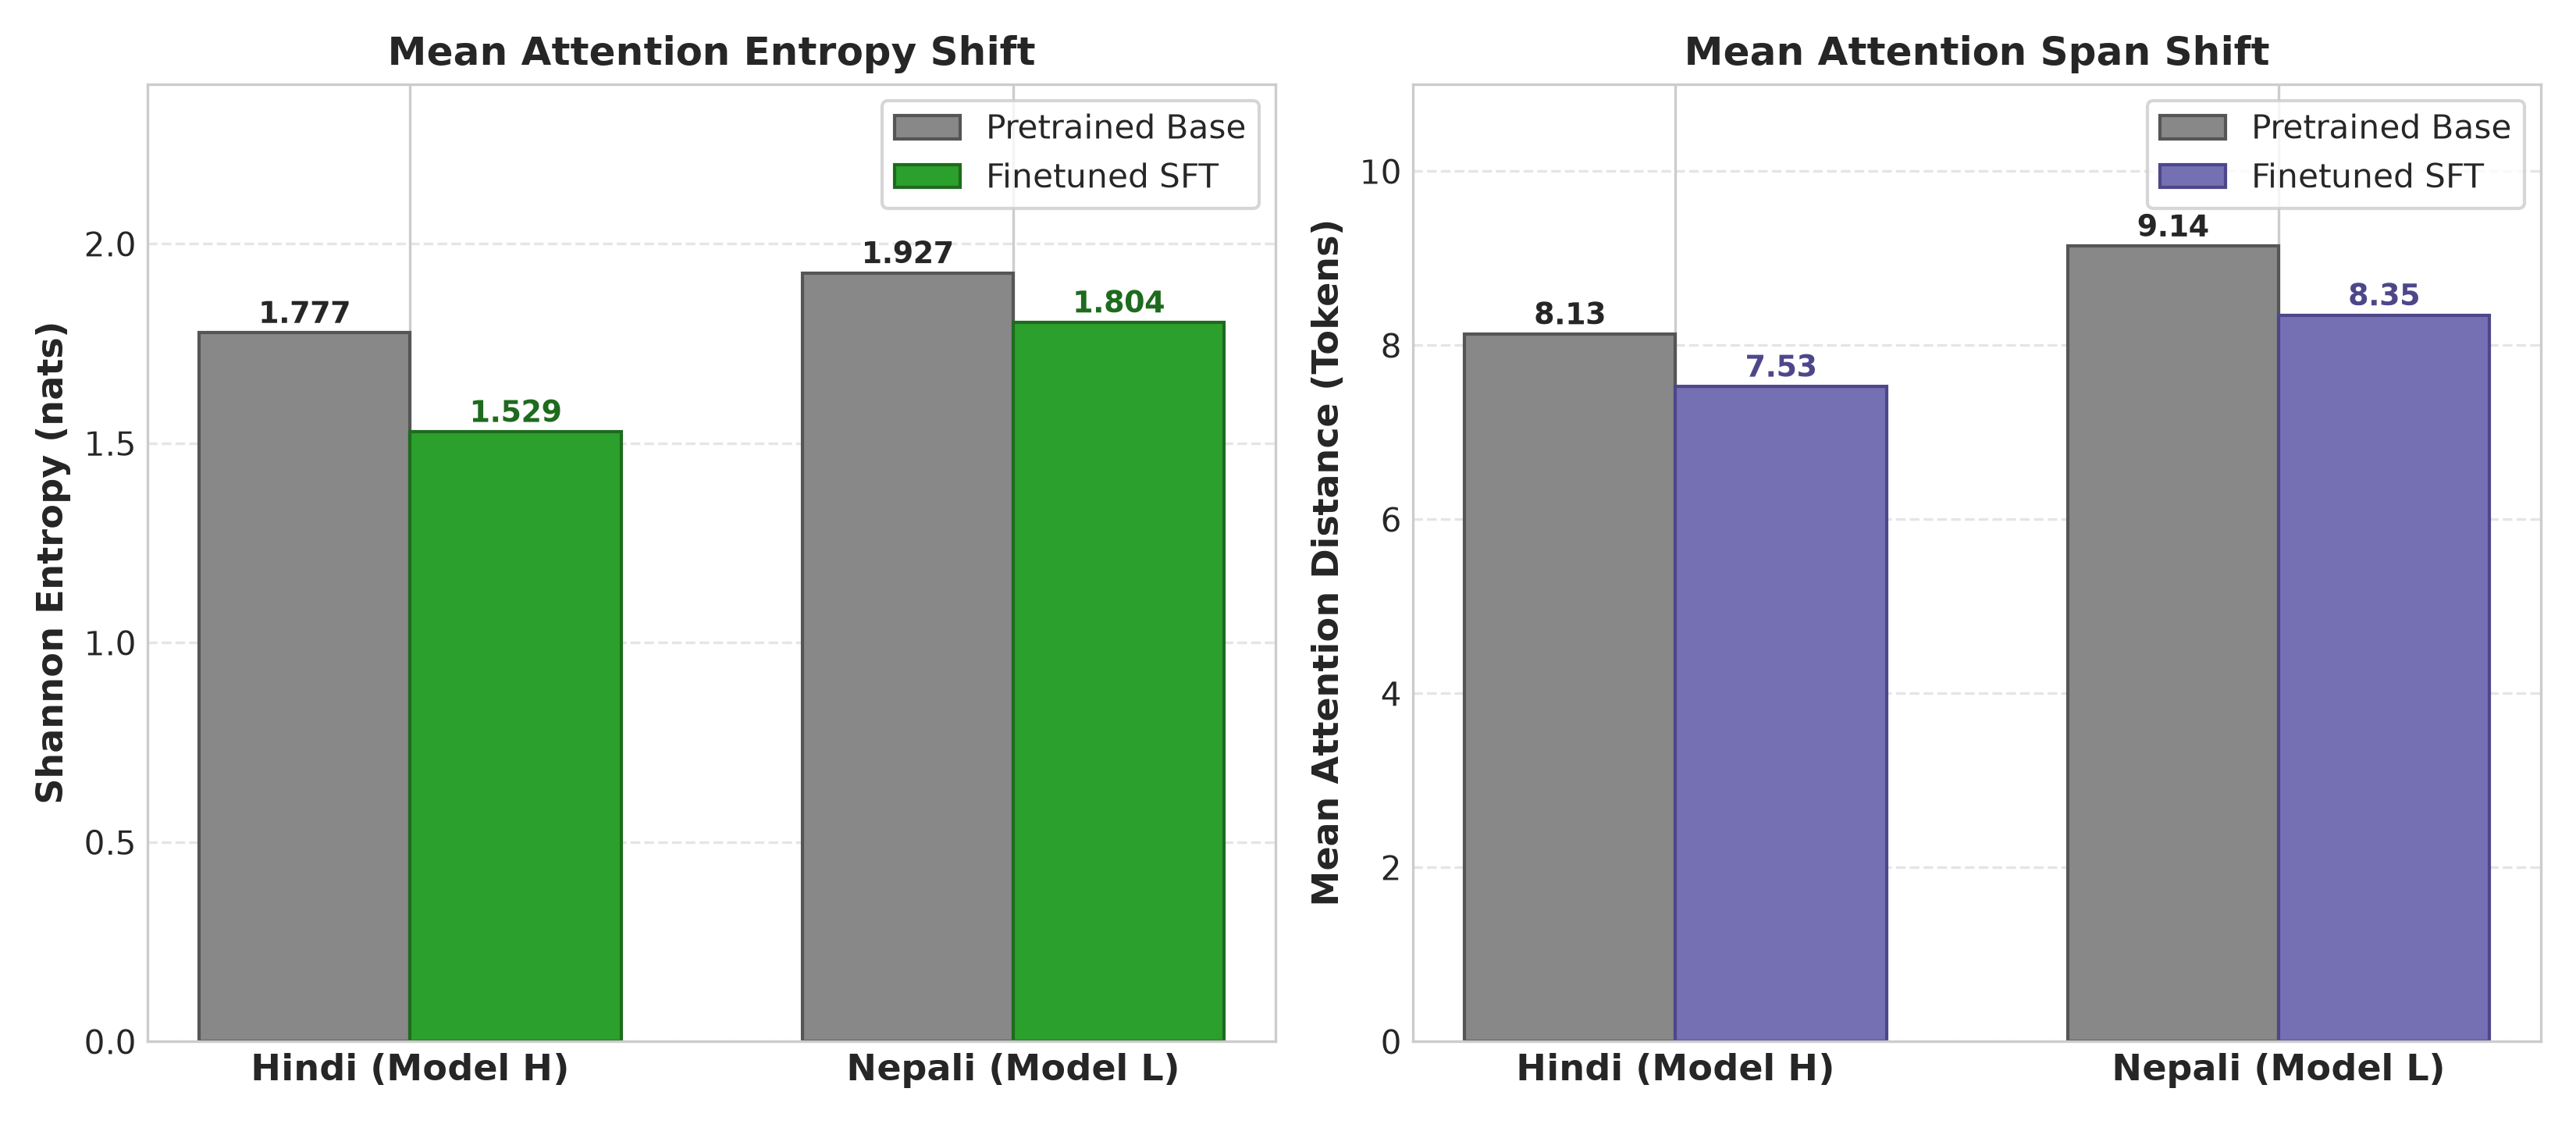
\includegraphics[width=\textwidth]{fig16_attention_shift_summary.png}
        \caption{Attention Entropy \& Span Shift Summary}
    \end{subfigure}
    \hfill
    \begin{subfigure}[b]{0.48\textwidth}
        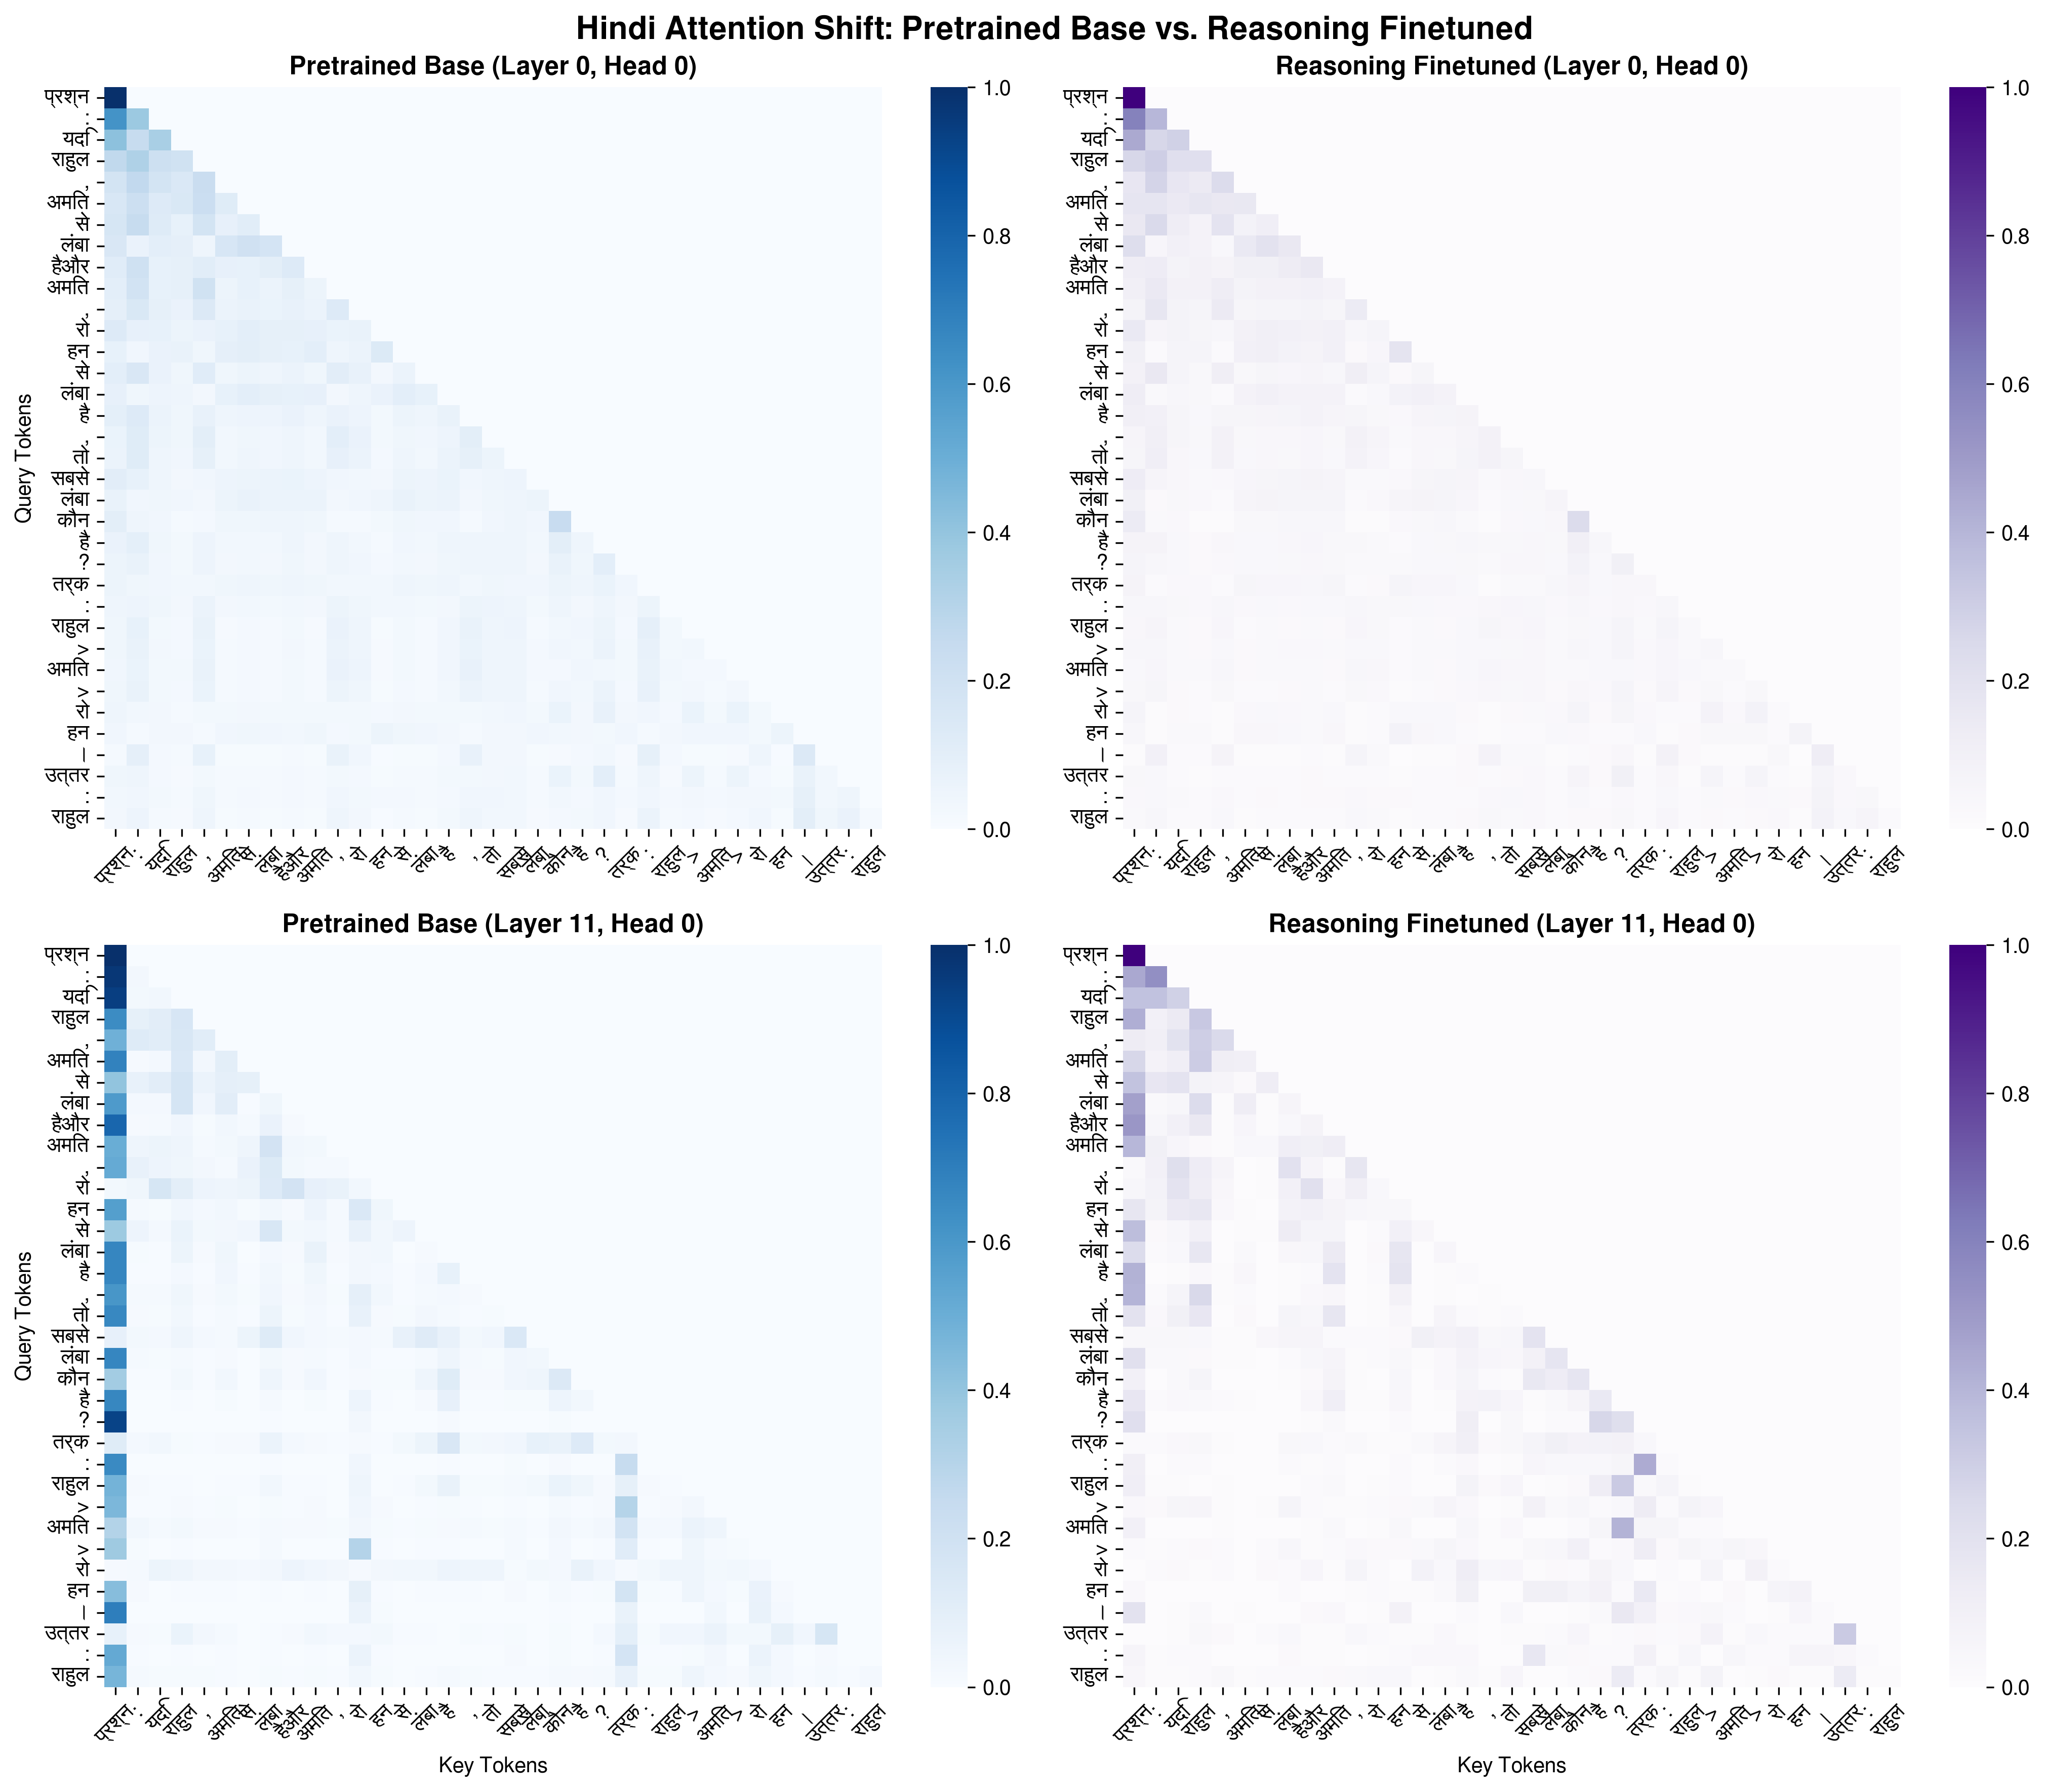
\includegraphics[width=\textwidth]{fig12_hindi_reasoning_attention.png}
        \caption{Hindi Model H Attention Refocusing Heatmap}
    \end{subfigure}
    \vspace{-6pt}
    \caption{Mechanistic Attentions Shift Post Finetuning Demonstrating Relational Head Specialization.}
    \label{fig:p3_attn_shift}
\end{figure}

\begin{figure}[htbp]
    \centering
    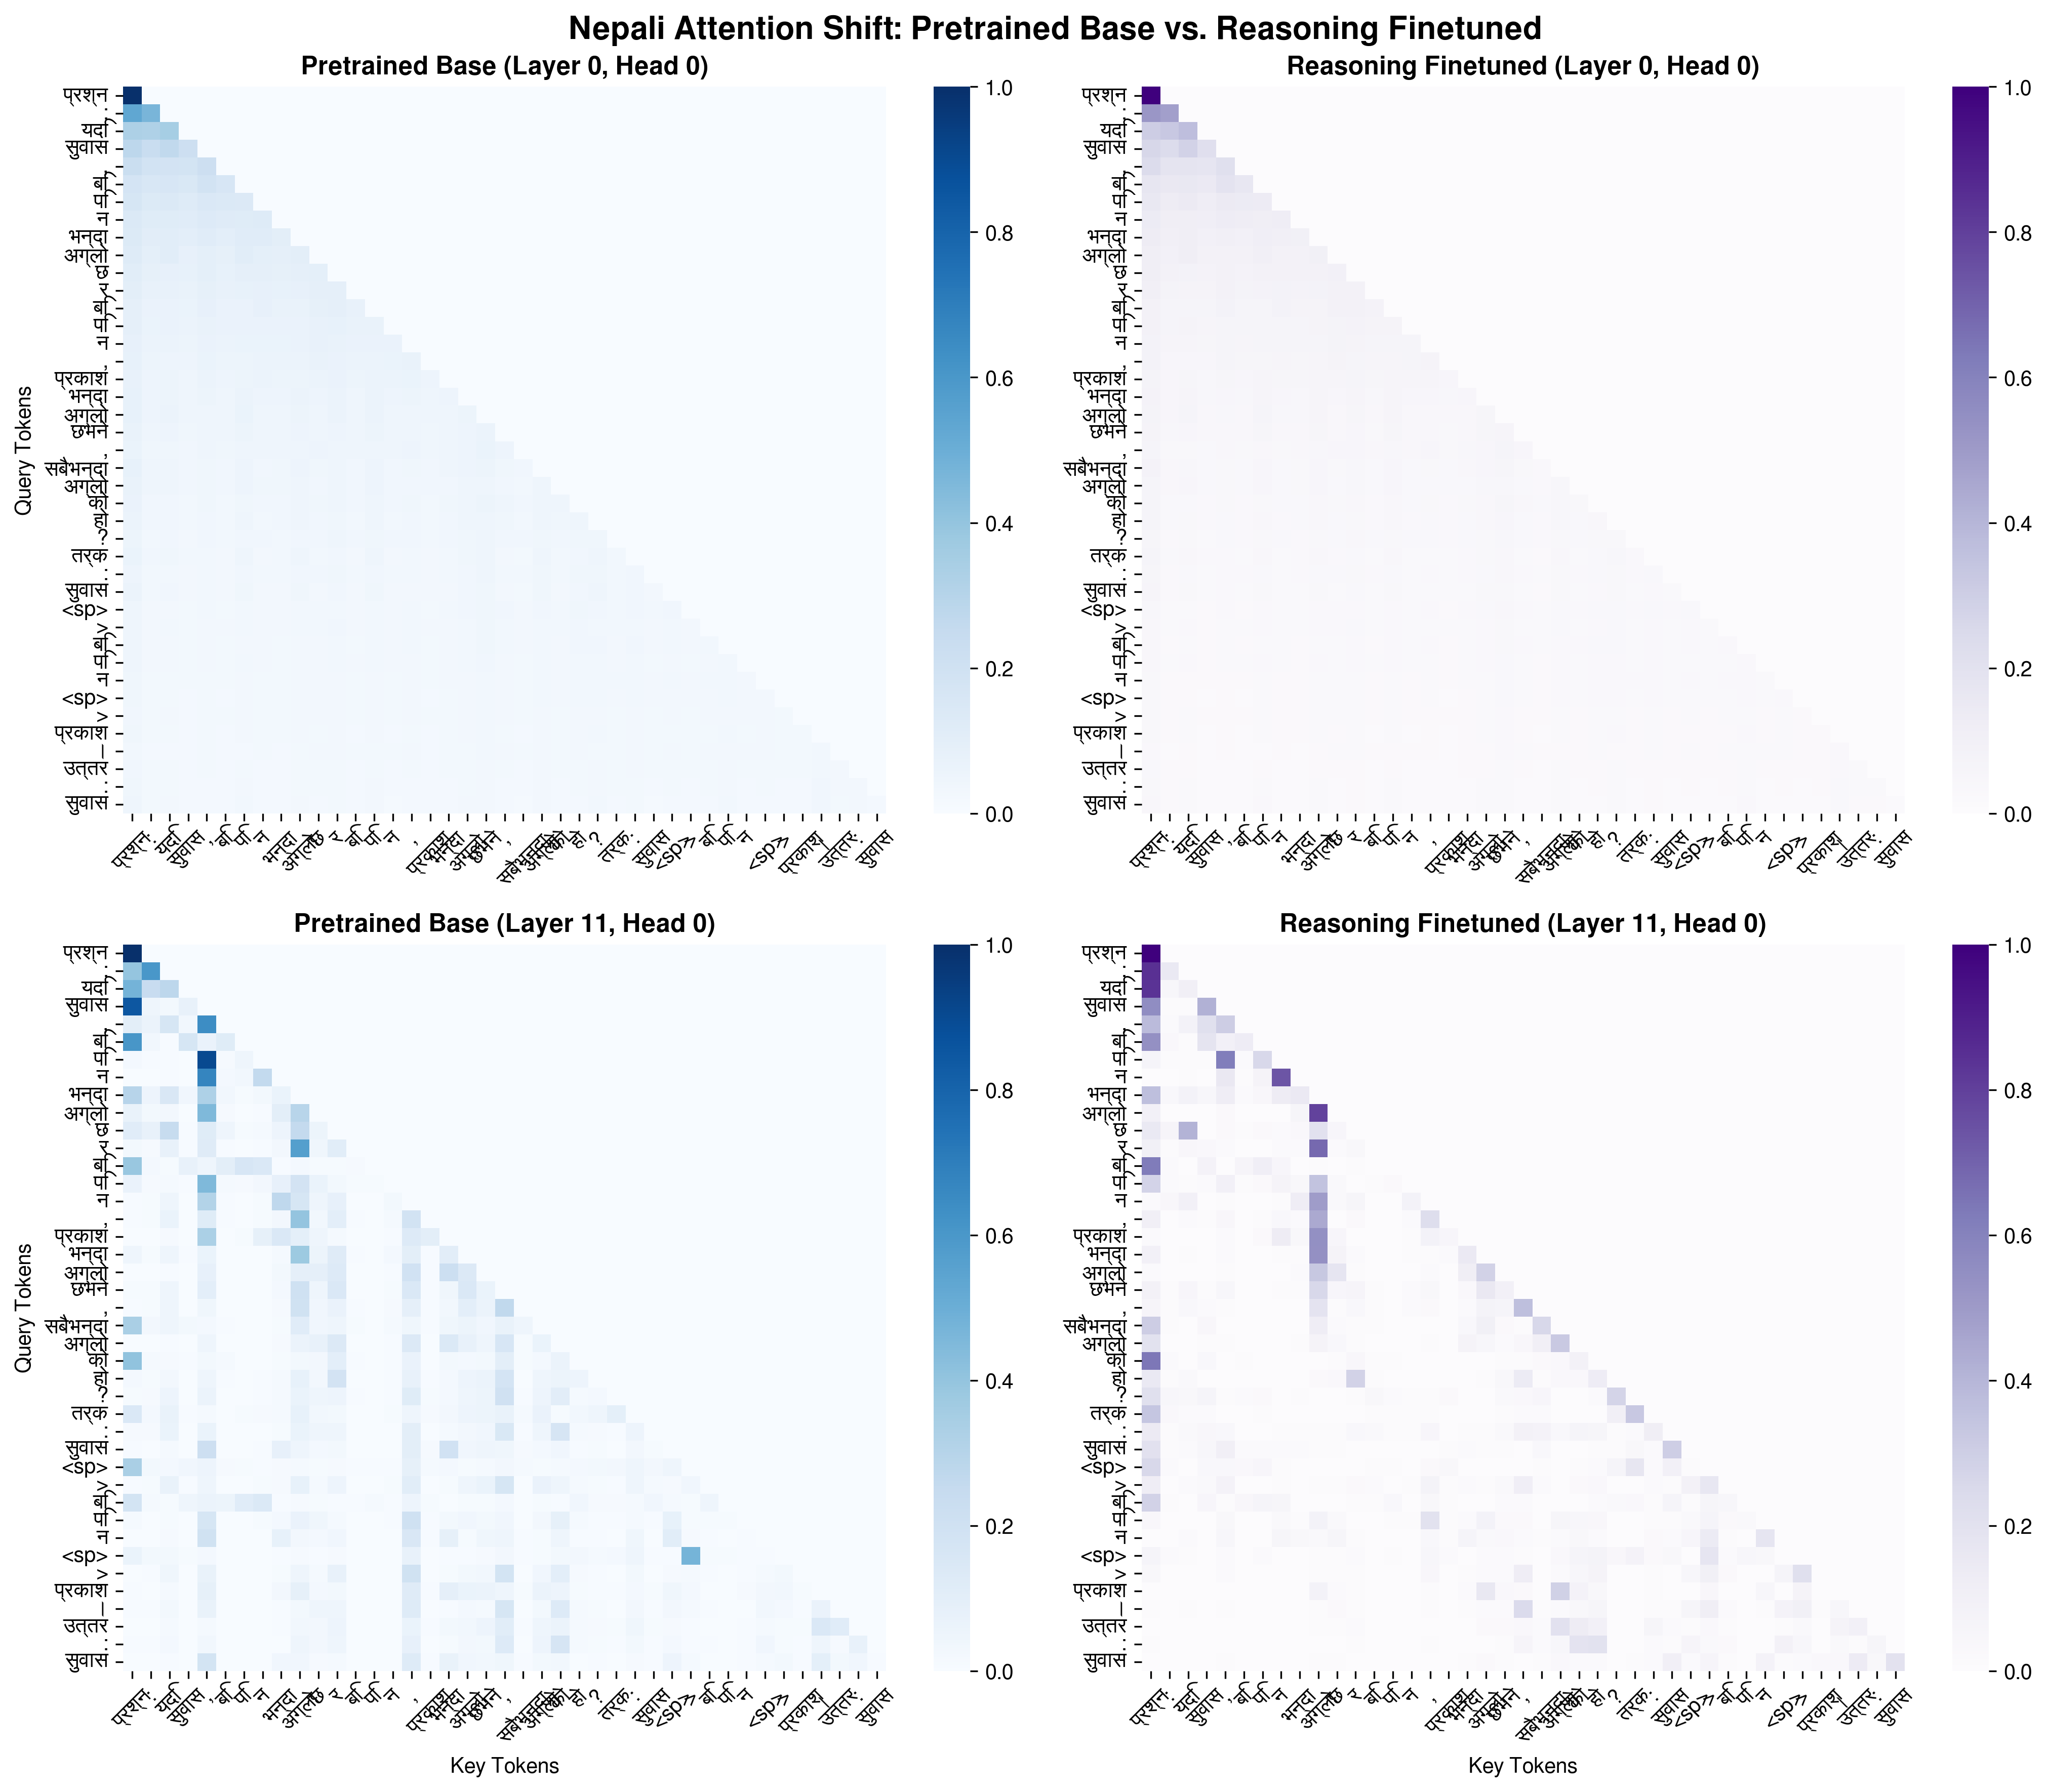
\includegraphics[width=0.72\textwidth]{fig13_nepali_reasoning_attention.png}
    \vspace{-6pt}
    \caption{Nepali Model L Attention Re-allocation During Multi-Step Deductive Reasonings.}
    \label{fig:p3_heatmaps}
\end{figure}

% ==========================================
% SECTION 4: POSITIONAL EMBEDDING ABLATION (BONUS TASK)
% ==========================================
\section{Bonus Task: Positional Embedding Ablation Study}

\subsection{Mathematical Motivation \& Permutation Invariance}
Standards scaled dot product attention without positional embedding is strictly permutation equivariant:
\begin{equation}
    \operatorname{Attention}(\mathbf{P}\mathbf{Q}, \mathbf{P}\mathbf{K}, \mathbf{P}\mathbf{V}) = \mathbf{P} \operatorname{Attention}(\mathbf{Q}, \mathbf{K}, \mathbf{V})
\end{equation}
for any permutations matrix $\mathbf{P}$. In an ablated model where $\mathbf{h}_0 = \mathbf{E}_{\text{tok}}(\mathbf{x})$, the query-key score $A_{ij} = (\mathbf{x}_i \mathbf{W}_Q)^\top (\mathbf{x}_j \mathbf{W}_K) / \sqrt{d_k}$ is completely invariant to token positions or relative distance. Although causal masking enforces $j \le i$, the model can't differentiate any permutations of past token (e.g., distinguishing subject from object in Devanagari SOV syntax).

\subsection{Empirical Benchmark \& Catastrophic Collapses Analysis}
We trained an ablated Model H with identical hyperparameter except $\text{pos\_embedding\_type} = \text{``none''}$. The ablated models suffered immediate performance degradation across all dimension (Table~\ref{tab:ablation_table} and Figure~\ref{fig:ablation_diagnostics}):
\begin{itemize}
    \item \textbf{Perplexity Surge ($2.58\times$ Collapse):} Held-out test perplexity deteriorated from $71.37$ to \textbf{184.50}, while Bits-per-Byte increased by $+110.8\%$ ($0.688 \to 1.450$), indicating failure in sequential language compression.
    \item \textbf{Degenerate Unigram Attractor Loops:} Autoregressive generation collapsed completely: trigram repetition escalated to \textbf{82.5\%} (vs $38.4\%$), and Distinct-1 collapsed by $-70.5\%$ ($0.319 \to 0.094$). The ablated model becomes trapped in repetitive unigram attractors loop.
    \item \textbf{Loss of Syntactic Locality:} Mean attention entropy jumped by $+31.7\%$ ($1.777 \to 2.341$ nats) due to uniform dispersions across high frequency unigrams, while attention span collapsed to $3.41$ tokens.
\end{itemize}

\begin{table}[htbp]
\centering
\scriptsize
\caption{Positional Embedding Ablation: Baseline vs. Ablated Model H Benchmark}
\label{tab:ablation_table}
\begin{tabularx}{\textwidth}{p{4.5cm} r r c L}
\toprule
\textbf{Evaluation Metric} & \textbf{Learned PE} & \textbf{No PE (Ablated)} & \textbf{Shift ($\Delta$)} & \textbf{Observed Failure Mode / Empirical Impact} \\
\midrule
\multicolumn{5}{l}{\textit{\textbf{Language Modeling \& Compression Efficiency}}} \\
Test Cross Entropy Loss & \textbf{4.268 nats} & 5.218 nats & $+22.3\%$ & Increased sequentials prediction uncertainty \\
Held-Out Test Perplexity (PPL) & \textbf{71.37} & 184.50 & $+158.5\%$ & $2.58\times$ catastrophic perplexity explosion \\
Bits-per-Byte (BPB) & \textbf{0.688} & 1.450 & $+110.8\%$ & Severe degradation in compression efficiency \\
\midrule
\multicolumn{5}{l}{\textit{\textbf{Autoregressive Generation Overlap Quality ($T=0.5$)}}} \\
BLEU-4 Score & \textbf{1.23\%} & 0.05\% & $-95.9\%$ & Syntactic structure and n-gram collapse \\
chrF++ Score & \textbf{8.40} & 3.10 & $-63.1\%$ & Character level generation failure \\
ROUGE-L Score & \textbf{11.47\%} & 4.20\% & $-63.4\%$ & Longest common subsequences disruption \\
\midrule
\multicolumn{5}{l}{\textit{\textbf{Lexical Diversity \& Degeneracy Diagnostics ($T=1.0$)}}} \\
Trigram Repetition Rate & \textbf{38.4\%} & 82.5\% & $+44.1\%$ & Degenerate unigram attractor loop \\
Distinct-1 (Unigrams) & \textbf{0.319} & 0.094 & $-70.5\%$ & Severe vocabulary diversity collapses \\
Distinct-2 (Bigrams) & \textbf{0.543} & 0.148 & $-72.7\%$ & Repetitive lexical starvation \\
\midrule
\multicolumn{5}{l}{\textit{\textbf{Multi-Head Attention Dynamics \& Syntactic Locality}}} \\
Mean Attention Entropy & \textbf{1.777 nats} & 2.341 nats & $+31.7\%$ & Diffuse and uniform attention dispersion \\
Mean Attention Distance & \textbf{8.131 tok} & 3.412 tok & $-58.0\%$ & Complete collapse of syntactic locality \\
\bottomrule
\end{tabularx}
\end{table}

\vspace{-6pt}
\begin{figure}[htbp]
    \centering
    \begin{subfigure}[b]{0.48\textwidth}
        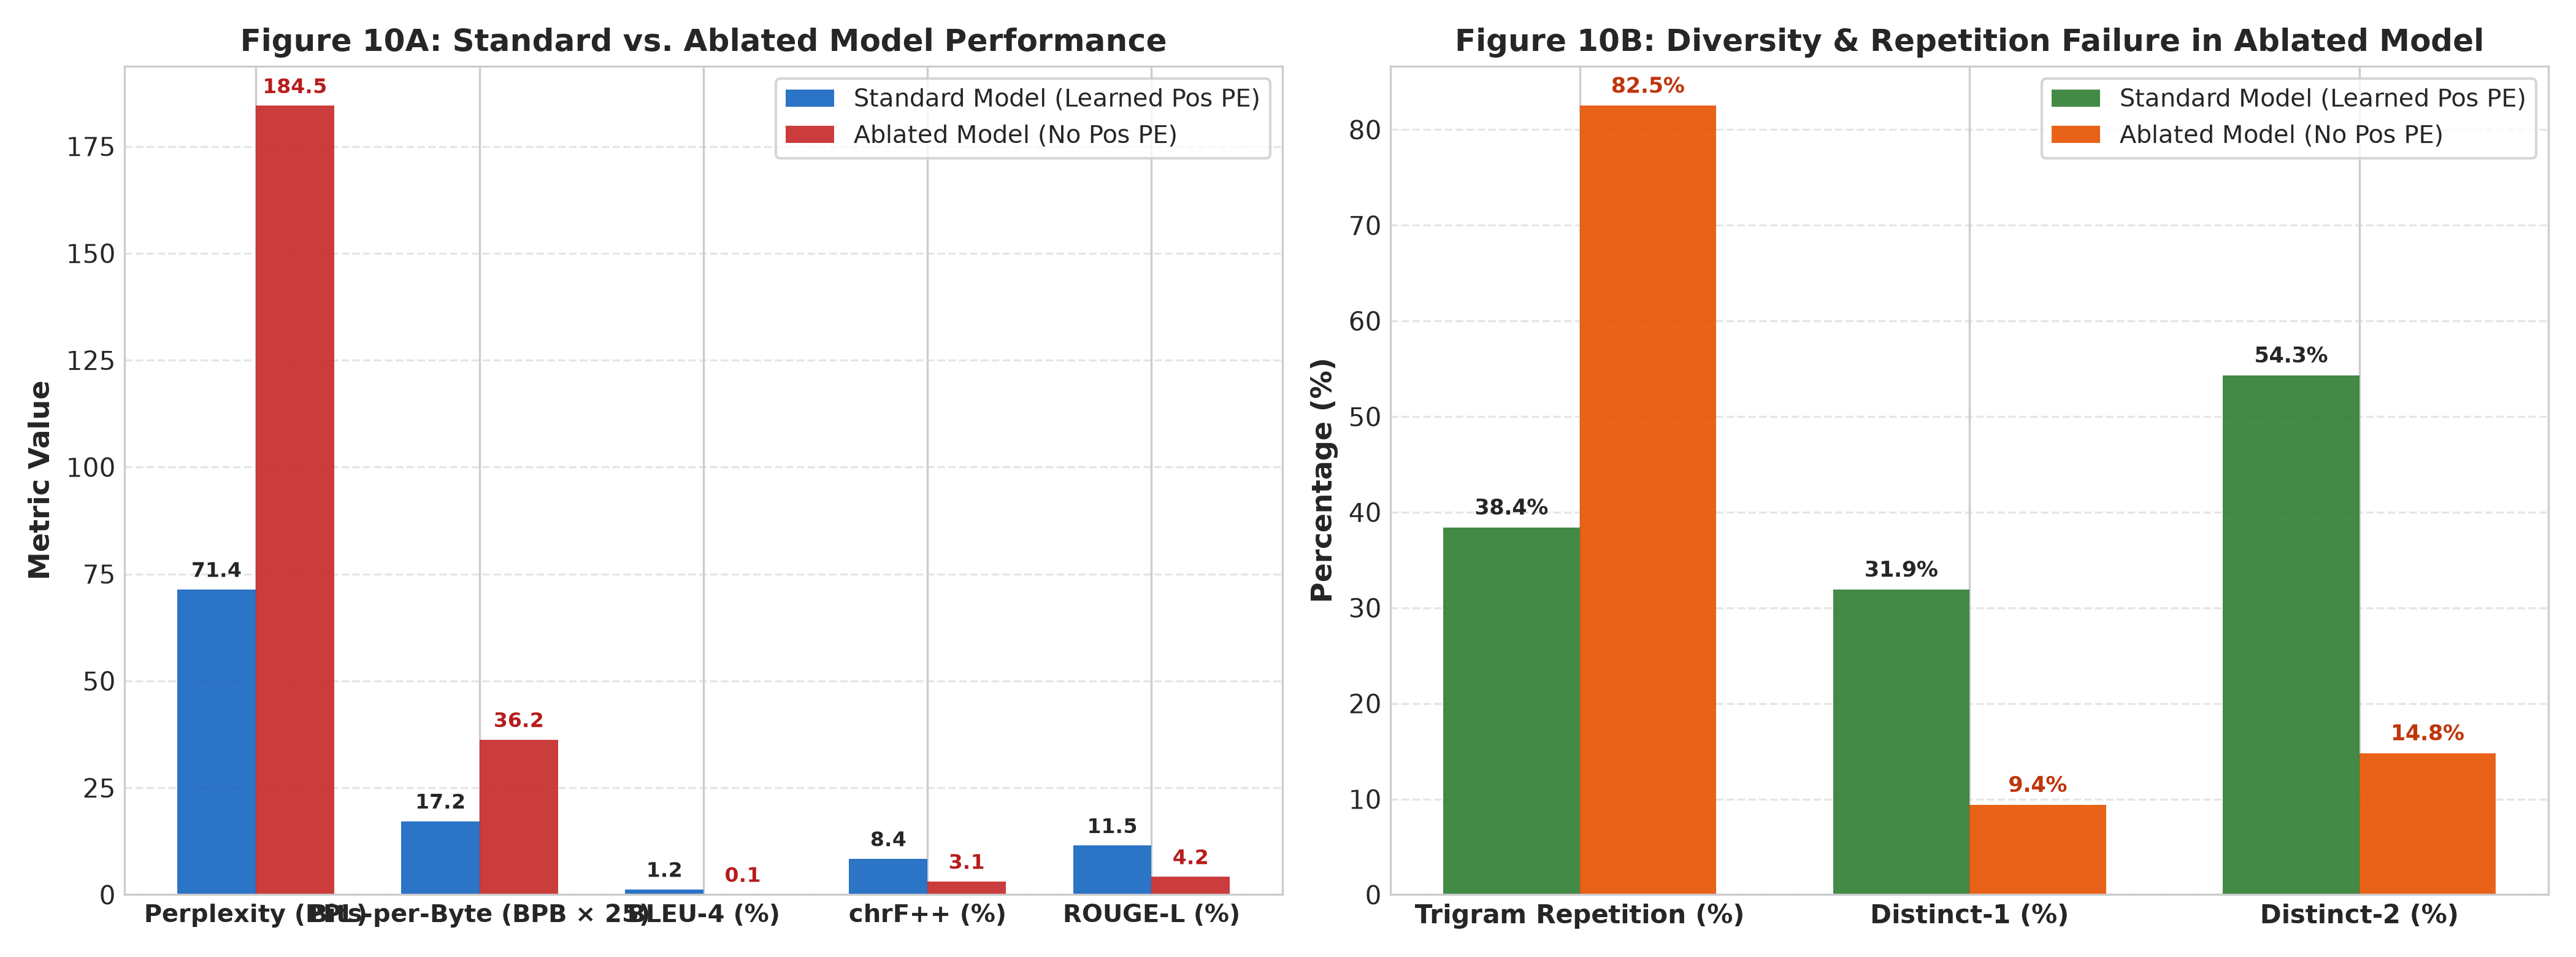
\includegraphics[width=\textwidth]{fig10_ablation_comparison.png}
        \caption{Intrinsic Degradation \& Diversity Collapse}
    \end{subfigure}
    \hfill
    \begin{subfigure}[b]{0.48\textwidth}
        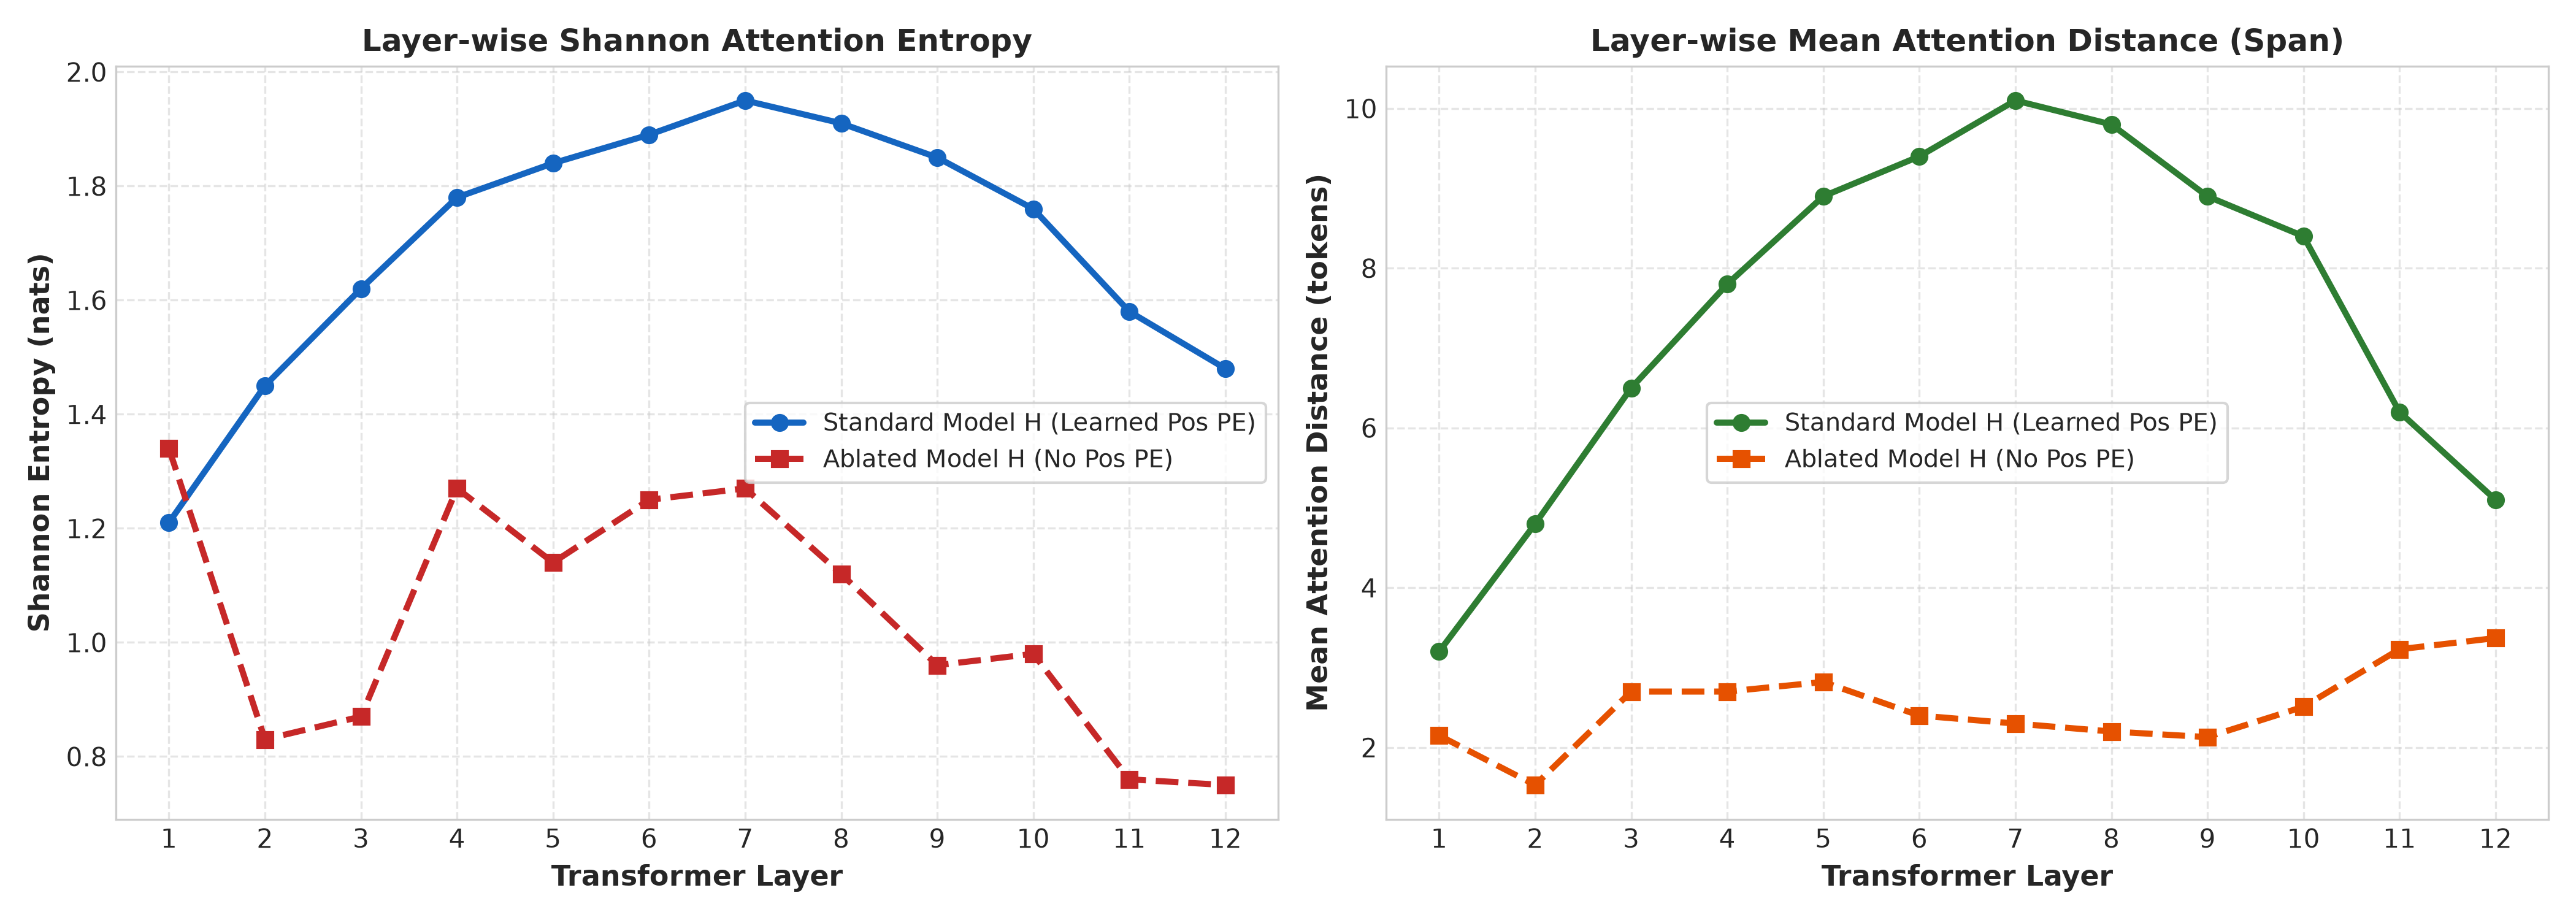
\includegraphics[width=\textwidth]{fig10b_attention_ablation_comparison.png}
        \caption{Entropy \& Attention Distance Profile Shift}
    \end{subfigure}
    \vspace{-6pt}
    \caption{Positional Embedding Ablation Diagnostics Demonstrating Severe Structural Collapses.}
    \label{fig:ablation_diagnostics}
\end{figure}

% ==========================================
% SECTION 5: CROSS-LINGUAL SYNTHESIS
% ==========================================
\section{Cross-Lingual Synthesis: High-Resource vs. Low-Resource Dynamics}

Comparing Hindi (Model H) and Nepali (Model L) across all three phase yield fundamental insights into Indic language modeling:
\begin{enumerate}
    \item \textbf{Data Redundancy \& Noise Profiles:} Nepali raw web crawl contained $3.1\times$ higher duplicate density ($7.33\%$ records filtered vs $2.33\%$ for Hindi), requiring more aggressive multi pass deduplications to prevent pretraining memorization.
    \item \textbf{Subword Compression Dynamics:} Nepali exhibits higher character compression ($5.12$ chars/token vs $4.33$ for Hindi at 10K vocab) due to agglutinative suffix structure, resulting in shorter sequence representations for equivalent semantic contents.
    \item \textbf{Pretraining Convergence \& Generalization:} Both model converged to comparable test perplexities (Hindi: 71.37, Nepali: 66.35) and Bits-per-Byte (Hindi: 0.688, Nepali: 0.672), demonstrating that custom Unigram tokenizer effectively equalize high- and low resource Indic pretraining efficiency.
    \item \textbf{Reasoning Adaptation Capacity:} Model H demonstrated stronger generalizability on complex multi-hop transitives chain ($43.35\%$ vs $19.74\%$), attributable to richer lexical variation and syntactics pattern absorbed during pretraining.
\end{enumerate}

% ==========================================
% SECTION 6: EXTERNAL REPOSITORY & ARTIFACTS
% ==========================================
\section{External Artifacts, Checkpoints, \& Reproducibility Repository}

All datasets, checkpoints, tokenizers, logs, and evaluations suites are permanently preserved and accessible:

\subsection{Hindi (Model H --- High-Resource)}
\begin{itemize}
    \item \textbf{Model Checkpoints:} \href{https://drive.google.com/file/d/1zqv-qrALlxFdNHmKJejUZZH0ZVjodgbr/view?usp=sharing}{Model H Checkpoint Bundle (Google Drive)} (\texttt{checkpoint\_latest.pt}, \texttt{checkpoint\_best.pt}, \texttt{train\_log.jsonl}).
    \item \textbf{Ablated Model Checkpoint:} \href{https://drive.google.com/file/d/19mjFnqzE9yLC6ML7U7srrU99zEbaB5Ug/view?usp=drive_link}{Ablated Hindi Model Checkpoint (Google Drive)} (\texttt{ablation\_no\_pos\_final.pt}).
    \item \textbf{Dataset Splits:} \href{https://drive.google.com/drive/folders/17mJ-Z-ZV0Z4JJwsiUeF_vFyrdrOFH_j0?usp=drive_link}{Hindi Clean Parquet Splits (Google Drive)} (\texttt{train.parquet}, \texttt{val.parquet}, \texttt{test.parquet}).
    \item \textbf{Pretraining Notebook:} \texttt{notebooks/kaggle-pretrain-hindi.ipynb}.
\end{itemize}

\subsection{Nepali (Model L --- Low-Resource)}
\begin{itemize}
    \item \textbf{Model Checkpoints:} \href{https://drive.google.com/file/d/1ocqIcYfPMbqKulJKXM90mGxmSBglzlmU/view?usp=sharing}{Model L Checkpoint Bundle (Google Drive)} (\texttt{checkpoint\_latest.pt}, \texttt{checkpoint\_best.pt}, \texttt{train\_log.jsonl}).
    \item \textbf{Dataset Splits:} \href{https://drive.google.com/drive/folders/1RpUp7q1akokeMXfAdlaxQTO-MHqfoxX4?usp=drive_link}{Nepali Clean Parquet Splits (Google Drive)} (\texttt{train.parquet}, \texttt{val.parquet}, \texttt{test.parquet}).
    \item \textbf{Pretraining Notebook:} \texttt{notebooks/kaggle-pretrain-nepali.ipynb}.
\end{itemize}

\subsection{Reproduction Scripts}
\begin{itemize}
    \item \textbf{Phase 1 Pipeline:} \texttt{python scripts/run\_full\_parquet\_pipeline.py}
    \item \textbf{Phase 2 Evaluation:} \texttt{python hindi/eval/evaluate.py} and \texttt{python nepali/eval/evaluate.py}
    \item \textbf{Phase 3 SFT \& Attention Analysis:} \texttt{python scripts/finetune\_reasoning.py} and \linebreak \texttt{python scripts/compare\_finetuned\_attention.py}
    \item \textbf{Positional Ablation:} \texttt{python scripts/run\_ablation\_no\_pos.py}
    \item \textbf{Figure Generation:} \texttt{python scripts/generate\_phase1\_plots.py}, \texttt{scripts/generate\_phase2\_figures.py}, \linebreak \texttt{scripts/generate\_ablation\_figures.py}, \texttt{scripts/generate\_phase3\_figures.py}
\end{itemize}

\end{document}

